% setenv TEXINPUTS .:/home/neyer/tex:/pub/blabla/tex:
% setenv LATEX_CONV_CONFIG /pub/blabla/CGAL/Tools/latex_converter_config
% setenv LATEX_CONV_HEADER /pub/blabla/CGAL/CGAL/include
% setenv LATEX_CONV_BIN /pub/blabla/sun4OS5/bin

%\documentclass[12pt]{book}
%\usepackage{latexsym}
%\usepackage{amssymb}
%\usepackage{path}
%\usepackage{epsfig}
%\usepackage{makeidx,psfrag}
%\makeindex
%
%%%%\pagestyle{empty}
%\textwidth 15.4cm 
%\textheight 24 cm
%\topmargin -14mm       
%\evensidemargin 3mm 
%\oddsidemargin 3mm
% 
%% ----------------------------------------
% new commands needed in the new mechamism
% 03.08.1995   Berlin   Lutz Kettner
% $Revision$
% $Date$
% ----------------------------------------

\tracingmacros=1
\newcount\nestinglevel  % counts nesting levels of template parameters
\newcount\xnestinglevel % counts nesting levels of template parameters
\newcount\spaceflag     % result, weather a parameter starts with a space
\newcount\emptyflag     % result, weather a parameter is empty (besides spaces)

\newcount\NParameters   % counts number of parameters for operators
\newbox\parameterX      % first parameter
\newbox\parameterXX     % second parameter
\newbox\parameterXXX    % third and rest of parameters

\def\CCfont{\em}        % font or style changing command in which all C++
                        % tokens will be typeset, including the variable names.
\def\CCendfont{\/}      % will be used after a C++ text. For slanted fonts,
                        % here should stay \/ macro.

\def\CCopenangle  {\CCendfont {\tt <}}
\def\CCcloseangle {\CCendfont {\tt >}}
\def\CCampersand  {\CCendfont {\tt \&}}
\def\CCunderscore {\_}

% These macros allow the characterwise parsing of an argument, where normally
% the spaces are ignored.
% Here, the first macro can be applied to the rest of the argument and 
% will return 1 in the \spaceflag iff the rest starts with a space.
% The second macro will produce a space "\ " iff the rest starts with a space.
% The space of the rest will be skipped automatically in the next round.
\def\testSpace #1{%
    \def\qparams{#1}\ifx\qparams\empty\spaceflag=0 
        \else\compareSpace{#1}#1\end\fi}
\def\compareSpace #1#2#3\end{%
    \def\xxparams{#1}\def\xxxparams{#2#3}\ifx\xxparams\xxxparams\spaceflag=0
        \else\spaceflag=1 \fi}
\def\testAndCopySpace #1{%
    \def\qparams{#1}\ifx\qparams\empty\else\compareAndCopySpace{#1}#1\end\fi}
\def\compareAndCopySpace #1#2#3\end{%
    \def\xxparams{#1}\def\xxxparams{#2#3}\ifx\xxparams\xxxparams\else\ \fi}

% This macro test wheather its argument is empty or contains only spaces.
\def\testEmpty #1{%
    \testEmptyX #1;\end}
\def\testEmptyX #1#2\end{%
    \def\xparams{#2}\ifx\xparams\empty\emptyflag=1 \else\emptyflag=0 \fi}

\newenvironment{class}[1]{%
                   \gdef\pureclassname{#1}%
                   \gdef\puretemplatename{#1}%
                   \gdef\pureparameters{}%
                   \gdef\classname{\hbox{{\CCfont 
                           \CCprintTokens #1\end\CCendfont}}}%
                   \gdef\classtemplatename{\hbox{{\CCfont
                           \CCprintTokens #1\end\CCendfont}}}%
                   }{}

\newenvironment{classtemplate}[2]{%
                   \gdef\pureclassname{#1}%
                   \gdef\puretemplatename{#1<#2>}%
                   \gdef\pureparameters{#2}%
                   \gdef\classname{\hbox{{\CCfont
                           \CCprintSingleToken #1;\CCendfont}}}%
                   \gdef\classtemplatename{\hbox{{\CCfont
                           \CCprintTokens #1\end}%
                           \CCendfont{\tt <}{\CCfont #2}\CCendfont{\tt >}}}%
                   }{}

\def\CCsection #1{%
                   \section[#1 (\protect\CCprintSingleToken \pureclassname;)]%
                           {#1 (\classname)}
                   \label{#1}}

\def\creationvariable #1{%
                   \gdef\var{$#1$}
                   \gdef\purevar{#1}}

\def\threecolumns #1#2{\typewidth=#1
                   \callwidth=#2
                   \descriptwidth=\textwidth
                   \advance\descriptwidth-\typewidth
                   \advance\descriptwidth-\callwidth
                   \advance\descriptwidth-0.5cm
                   \callwidthl=\textwidth 
                   \advance\callwidthl-\typewidth
                   \advance\callwidthl-0.5cm
                   }


% Print a character of a C++ declaration. Special handling of _<>&.
\def\CCprintChar #1{%
                   \if_#1\CCunderscore
                   \else\if<#1\CCopenangle
                   \else\if>#1\CCcloseangle
                   \else\if&#1\CCampersand
                   \else #1%
                   \fi\fi\fi\fi}

% Print a single C++ token (without spaces inbetween). Skip leading spaces.
% The token has to be delimited by a ";".
\def\CCprintSingleToken #1#2;{%
                   \CCprintChar #1%
                   \def\xparams{#2}%
                   \def\xbody{\CCprintSingleToken #2;}%
                   \ifx\xparams\empty\let\xnext=\relax
                   \else\let\xnext=\xbody\fi
                   \xnext}

% Print C++ tokens (separated with spaces). Skip leading spaces.
% The tokens have to be delimited by "\end".
\def\CCprintTokens #1#2\end{%
                   \CCprintChar #1%
                   \def\xbody{\CCprintTokens #2\end}%
                   \testEmpty{#2}\ifnum\emptyflag=1
                       \let\xnext=\relax
                   \else
                       \compareAndCopySpace{#2}#2\end
                       \let\xnext=\xbody
                   \fi
                   \xnext}

% Print one parameter in C++ style (including spaces).
\def\CCstyle #1{{\CCfont \CCprintTokens #1\end\CCendfont}}

% Print a parameter where "const ...&" pairs are eliminated. Strips a
% leading type that equals the \classname. It is a three step process:
%   1. strip all in front of a "<" character.
%   2. extract the leading token without any space in it to decide,
%      weather the type given is a templated type or not.
%   3. Compare the leading token with \classname
%   4. If true, strip the possible following template parameter.
% The parameter has to be delimited with "<>;".
% Ignore leading spaces.
\def\CCprintOwnClassParameter #1#2<#3#4;{%
        \ifx\pureparameters\empty
            \CCprintOwnClassX  #1#2 ;% no template case
        \else\if>#3%
            \CCprintOwnClassX  #1#2 ;% no template case
        \else
            \CCprintOwnClassXX{#1#2}<#3#4;% template case ?
        \fi\fi}
\def\CCprintOwnClassX #1 #2;{% check for \classname
        \def\xparams{#1}\ifx\xparams\pureclassname
            \CCprintTokens #2\end%
        \else
            \CCprintTokens #1 #2\end%
        \fi}
\def\CCprintOwnClassXX #1#2<>;{% strip the unneccessary <> from the end
        \CCprintOwnClassXXX {#2}#1 ;}
\def\CCprintOwnClassXXX #1#2 #3;{%
        % check \classname in the possible template case
        %   #1 is the parameter tail starting with the template params
        %   #2 is the leading class name
        %   #3 is inbetween and should be empty
        \def\qqparams{#3}\ifx\qqparams\empty
            \def\xparams{#2}\ifx\xparams\pureclassname
                \xnestinglevel=0
                \CCprintOwnClassXXXX #1;% strip the template parameters
            \else
                \CCprintTokens #2#1\end% nothing stripped
            \fi
        \else
            \errhelp{The allowed syntax is: name< params...}%
            \errmessage{Confusing class name with a space before 
                        the template parameters.}%
        \fi}
\def\CCprintOwnClassXXXX #1#2;{% strip a leading template parameter
                   \if<#1\advance\xnestinglevel by1  \fi
                   \if>#1\advance\xnestinglevel by-1 \fi
                   \ifnum\xnestinglevel=0
                       \CCprintTokens #2\end%
                       \let\xnext=\relax
                   \else
                       \def\xparams{#2}%
                       \ifx\xparams\empty
                           \errhelp{Look for mismatching angles.}%
                           \errmessage{Mismatching angles in template 
                                       parameter list.}%
                       \fi
                       \def\xbody{\CCprintOwnClassXXXX #2;}%
                       \let\xnext=\xbody
                   \fi
                   \xnext}



% Print a C++ function or method parameter. Strips a matching
% "const ...&" pair.
% The parameter has to be delimited with "const.&.;".
\def\CCprintParameter #1const#2#3&#4#5;{%
    \if.#2\CCprintOwnClassParameter #1<>;%
    \else
        \if&#2\CCprintParameter #1#3&#4#5;%
        \else
        \CCprintParameter #1#2#3 #4#5;%
        \fi
    \fi}

% Print a C++ function or method return type. Strips a matching
% "const ...&" pair.
% The parameter has to be delimited with "const.&.;".
\def\CCprintReturnType #1const#2#3&#4#5;{%
    \if.#2\CCprintTokens #1\end%
    \else
        \if&#2\CCprintReturnType #1#3&#4#5;%
        \else
        \CCprintReturnType #1#2#3 #4#5;%
        \fi
    \fi}

% Print a C++ parameter list (separated with commatas). The output formats
% with a space between commata and the parameter text.
\def\CCprintParamList #1{%
        \nestinglevel=0
        \CCprintParamListX{}#1;}
% Support function:
%   o  The first parameter accumulates the so far parsed first parameter.
%   o  The second parameter contains the next character.
%   o  The third parameter contains the rest.
% The parsing process iterates characterwise.
% The parameter list has to be terminated with ";".
\def\CCprintParamListX #1#2#3;{%
                   \testSpace{#3}%
                   \if<#2\advance\nestinglevel by1 \fi
                   \if>#2\advance\nestinglevel by-1 \fi
                   \if,#2%
                       \ifnum\nestinglevel=0 
                           \CCprintParameter #1const.&.;,\ %
                           \def\xxbody{\CCprintParamListX{}#3;}%
                       \else\ifnum\nestinglevel<0
                           \def\errhelp{Look for unbalanced angles in 
                           template types in the C++ parameter list.}%
                           \errmessage{Unbalanced angles detected.}%
                           \def\xxbody{\CCprintParamListX{}#3;}%
                       \else% comma within template parameter detected
                           \ifnum\spaceflag=1
                               \def\xxbody{\CCprintParamListX
                                   {#1#2 }#3;}%
                           \else
                               \def\xxbody{\CCprintParamListX
                                   {#1#2}#3;}%
                           \fi
                       \fi
                       \fi
                   \else\def\xxparams{#3}\ifx\xxparams\empty%
                       \ifnum\nestinglevel=0
                           \CCprintParameter #1#2const.&.;%
                       \else\def\errhelp{Look for unbalanced angles in 
                           template types in the C++ parameter list.}%
                           \errmessage{Unbalanced angles detected.}%
                       \fi
                       \def\xxbody{\CCprintParamListX{}#3;}%
                   \else
                       \ifnum\spaceflag=1
                           \def\xxbody{\CCprintParamListX
                               {#1#2 }#3;}%
                       \else
                           \def\xxbody{\CCprintParamListX
                               {#1#2}#3;}%
                       \fi
                   \fi
                   \fi
                   \def\xxparams{#3}\ifx\xxparams\empty\let\xxnext=\relax
                   \else\let\xxnext=\xxbody\fi
                   \xxnext}

% Extract up to three parameters from a C++ parameter list 
% (separated with commatas) within the \paramterX.. boxes.
\def\CCextractParamList #1{%
        \nestinglevel=0
        \NParameters=0
        \def\xparams{#1}\ifx\xparams\empty\else
            \CCextractParamListX{}#1;\fi}
% Support function:
%   o  The first parameter accumulates the so far parsed first parameter.
%   o  The second parameter contains the next character.
%   o  The third parameter contains the rest.
% The parsing process iterates characterwise.
% The parameter list has to be terminated with ";".
\def\CCextractParamListX #1#2#3;{%
                   \testSpace{#3}%
                   \if<#2\advance\nestinglevel by1 \fi
                   \if>#2\advance\nestinglevel by-1 \fi
                   \if,#2%
                       \ifnum\nestinglevel=0 
                           \advance\NParameters by1
                           \ifnum\NParameters=1 \setbox\parameterX=%
                                   \hbox{\CCprintParameter #1const.&.;}%
                               \def\xxxbody{\CCextractParamListX{}#3;}%
                           \else\advance\NParameters by1
                               \setbox\parameterXX=%
                                   \hbox{\CCprintParameter #1const.&.;}%
                               \setbox\parameterXXX=%
                                   \hbox{\CCprintParamList{#3}}%
                               \def\xxxbody{\relax}%
                           \fi
                       \else\ifnum\nestinglevel<0
                           \def\errhelp{Look for unbalanced angles in 
                           template types in the C++ parameter list.}%
                           \errmessage{Unbalanced angles detected.}%
                           \def\xxxbody{\CCextractParamListX{}#3;}%
                       \else% comma within template parameter detected
                           \ifnum\spaceflag=1
                               \def\xxxbody{\CCextractParamListX
                                   {#1#2 }#3;}%
                           \else
                               \def\xxxbody{\CCextractParamListX
                                   {#1#2}#3;}%
                           \fi
                       \fi
                       \fi
                   \else\def\xxxparams{#3}\ifx\xxxparams\empty%
                       \ifnum\nestinglevel=0
                           \advance\NParameters by1
                           \ifnum\NParameters=1 \setbox\parameterX=%
                                   \hbox{\CCprintParameter #1#2const.&.;}%
                           \else\ifnum\NParameters=2 \setbox\parameterXX=%
                                   \hbox{\CCprintParameter #1#2const.&.;}%
                           \else\setbox\parameterXXX=%
                                   \hbox{\CCprintParameter #1#2const.&.;}%
                           \fi\fi
                       \else\def\errhelp{Look for unbalanced angles in 
                           template types in the C++ parameter list.}%
                           \errmessage{Unbalanced angles detected.}%
                       \fi
                       \def\xxxbody{\CCextractParamListX{}#3;}%
                   \else
                       \ifnum\spaceflag=1
                           \def\xxxbody{\CCextractParamListX
                               {#1#2 }#3;}%
                       \else
                           \def\xxxbody{\CCextractParamListX
                               {#1#2}#3;}%
                       \fi
                   \fi
                   \fi
                   \def\xxxparams{#3}\ifx\xxxparams\empty\let\xxxnext=\relax
                       \else\let\xxxnext=\xxxbody\fi
                   \xxxnext}


\def\constructorcall #1(#2)#3 \par {%
                   \def\params{#2}\ifx\params\empty%
                   \mbox{\classtemplatename\ \ \CCfont\purevar ;}%
                   \else\mbox{\classtemplatename
                       \ \ {\CCfont \purevar(\CCprintParamList{#2});}}%
                   \fi\par }
\def\constructor #1#2{%
                       \constructorcall #1 \par
                       \hspace*{1cm}\hfill
                       \parbox[t]{\createtextwidth}{\sloppy #2}\par
                       \bigskip
                       }

% The method/fct. call is checked for the operator keyword.
%   o  The first parameter contains a 0 for a method call, a 1 for a function.
%   o  The second parameter contains the (maybe empty) parameter list.
%   o  The third to fifth parameters parse the name.
% The declaration has to be terminated with "operator;\end".
\def\CCcheckOperator #1#2#3operator#4#5\end{%
                       \if;#4\ifnum#1=0 \purevar.\fi
                           \CCprintSingleToken #3;%
                           (\def\params{#2}\ifx\params\empty
                               \else\CCprintParamList{#2}\fi
                           )%
                       \else
                           \ifnum#1=0
                               \CCprintOperator{#1}{\purevar,}{#2}#4#5\end
                           \else
                               \CCprintOperator{#1}{}{#2}#4#5\end
                           \fi
                       \fi}


% An operator is detected and can be printed.
%   o  The first parameter contains a 0 for a method call, a 1 for a function.
%   o  The second parameter contains the \purevar if it is a method.
%   o  The third parameter contains the (maybe empty) parameter list.
%   o  The fourth parameter is the first character of the operator.
%   o  The fifth parameter contains the rest of the operator.
%   o  The sixth parameter is the ";".
% The declaration ends with "operator;\end".
\newcount\operatorerror
\def\CCprintOperator #1#2#3#4#5operator#6\end{%
                       \CCextractParamList{#2#3}%
                       \operatorerror=1
                       \def\xparams{#5}%
                       \ifx\xparams\empty 
                           % single character operations
                           \ifcase\NParameters         % no parameter
                           \or                         % 1 parameter
                               \if~#4\CCoperatorpraefix{\tilde{}}\fi
                               \if!#4\CCoperatorpraefix{#4}\fi
                               \if-#4\CCoperatorpraefix{#4}\fi
                               \if+#4\CCoperatorpraefix{#4}\fi
                               \if&#4\CCoperatorpraefix{\mbox{{\CCfont
                                       \CCampersand}}}\fi
                               \if*#4\CCoperatorpraefix{#4}\fi
                           \or                         % 2 parameters
                               \if*#4\CCoperatorinfix{#4}\fi
                               \if/#4\CCoperatorinfix{\,#4}\fi
                               \if\%#4\CCoperatorinfix{#4}\fi
                               \if+#4\CCoperatorinfix{#4}\fi
                               \if-#4\CCoperatorinfix{#4}\fi
                               \if<#4\CCoperatorinfix{#4}\fi
                               \if>#4\CCoperatorinfix{#4}\fi
                               \if&#4\CCoperatorinfix{\mbox{{\CCfont
                                       \CCampersand}}}\fi
                               \if^#4\CCoperatorinfix{\hat{}}\fi
                               \if|#4\CCoperatorinfix{#4}\fi
                               \if=#4\CCoperatorinfix{#4}\fi
                               \if,#4\CCoperatorinfix{#4}\fi
                           \else                       % 3 parameters
                           \fi
                       \else
                           % two or more character operations
                           \CCprintOperatorTwo #4#5\end
                       \fi
                       \ifnum\operatorerror=1 \def\errhelp{Look out
                           for the legal operator overloading in C++.
                           Maybe, not all operators are currently supported
                           by this style, sorry.}\errmessage{Unknown operator
                           detected. Go ahead, and I format it as a 
                           function.}%
                           \CCprintSingleToken operator#4#5;%
                           (\def\params{#3}\ifx\params\empty
                               \else\CCprintParamList{#3}\fi
                           )%
                       \fi
                     }

% An operator with two or more characters is detected and can be printed.
%   o  The first parameter is the first character of the operator.
%   o  The second parameter is the second character of the operator.
%   o  The third parameter contains the rest of the operator.
% The declaration ends with "\end".
\def\CCprintOperatorTwo #1#2#3\end{%
                   \def\xparams{#3}%
                   \ifx\xparams\empty 
                       % two character operations
                       \ifcase\NParameters         % no parameter
                       \or                         % 1 parameter
                           \if-#1\if>#2\CCoperatorpostfix{\:#1\!\!\!#2}\fi\fi
                           \if(#1\if)#2\CCoperatorparX{(}{)}\fi\fi
                           \if+#1\if+#2\CCoperatorpraefix{#1\!#2}\fi\fi
                           \if-#1\if-#2\CCoperatorpraefix{#1\!#2}\fi\fi
                       \or                         % 2 parameters
                           \if[#1\if]#2\CCoperatorparXX{[}{]}\fi\fi
                           \if(#1\if)#2\CCoperatorparXX{(}{)}\fi\fi
                           \if+#1\if+#2\CCoperatorpostfix{#1\!#2}\fi\fi
                           \if-#1\if-#2\CCoperatorpostfix{#1\!#2}\fi\fi
                           \if>#1\if>#2\CCoperatorinfix{#1#2}\fi\fi
                           \if<#1\if<#2\CCoperatorinfix{#1#2}\fi\fi
                           \if<#1\if=#2\CCoperatorinfix{#1#2}\fi\fi
                           \if>#1\if=#2\CCoperatorinfix{#1#2}\fi\fi
                           \if=#1\if=#2\CCoperatorinfix{#1#2}\fi\fi
                           \if!#1\if=#2\CCoperatorinfix{#1#2}\fi\fi
                           \if&#1\if&#2\CCoperatorinfix{\mbox{{\CCfont
                                       \CCampersand}}\mbox{{\CCfont
                                       \CCampersand}}}\fi\fi
                           \if|#1\if|#2\CCoperatorinfix{#1#2}\fi\fi
                           \if*#1\if=#2\CCoperatorinfix{#1#2}\fi\fi
                           \if/#1\if=#2\CCoperatorinfix{#1#2}\fi\fi
                           \if\%#1\if=#2\CCoperatorinfix{#1#2}\fi\fi
                           \if+#1\if=#2\CCoperatorinfix{#1#2}\fi\fi
                           \if-#1\if=#2\CCoperatorinfix{#1#2}\fi\fi
                           \if&#1\if=#2\CCoperatorinfix{\mbox{{\CCfont
                                       \CCampersand}}#2}\fi\fi
                           \if|#1\if=#2\CCoperatorinfix{#1#2}\fi\fi
                           \if^#1\if=#2\CCoperatorinfix{\hat{}#2}\fi\fi
                       \else                       % 3 parameters
                           \if(#1\if)#2\CCoperatorparXXX{(}{)}\fi\fi
                       \fi
                   \else
                       % three or more character operations
                       \ifcase\NParameters         % no parameter
                       \or                         % 1 parameter
                           \if-#1\if>#2\CCoperatorpostfix{\:#1\!\!\!#2#3}\fi\fi
                       \or                         % 2 parameters
                           \if#1n\if#2e\CCoperatornew{#1#2#3}\fi\fi
                           \if#1d\if#2e\CCoperatordelete{#1#2#3}\fi\fi
                           \if>#1\if>#2\CCoperatorinfix{#1#2#3}\fi\fi
                           \if<#1\if<#2\CCoperatorinfix{#1#2#3}\fi\fi
                       \else                       % 3 parameters
                       \fi
                   \fi
                 }


\def\CCoperatorpraefix #1{%
    $#1 \mbox{\box\parameterX}$\operatorerror=0 }
\def\CCoperatorinfix #1{%
    $\mbox{\box\parameterX} #1 \mbox{\box\parameterXX}$\operatorerror=0 }
\def\CCoperatorpostfix #1{%
    $\mbox{\box\parameterX} #1$\operatorerror=0 }
\def\CCoperatorappend #1#2{%
    $\mbox{\box\parameterX} #1#2$\operatorerror=0 }
\def\CCoperatorparX #1#2{%
    \box\parameterX#1#2\operatorerror=0 }
\def\CCoperatorparXX #1#2{%
    \box\parameterX#1\box\parameterXX#2\operatorerror=0 }
\def\CCoperatorparXXX #1#2{%
    \box\parameterX\CCendfont#1\box\parameterXX,
    \box\parameterXXX#2\operatorerror=0 }
\def\CCoperatornew #1{%
    $ * \mbox{{\CCfont ptr\_}\box\parameterX} = \mbox{{\CCfont #1}
              \box\parameterX}$\operatorerror=0 }
\def\CCoperatordelete #1{%
    $ \mbox{{\CCfont #1} {\CCfont ptr\_}\box\parameterX}$\operatorerror=0 }

% The first argument accumulates the type until only one token 
% without separating spaces remains (i.e. the method name).
\def\extracttype #1#2 #3;{\def\params{#3}%
                       \ifx\params\empty \CCprintReturnType #1const.&.;%
                       \else\extracttype{#1 #2}#3;\fi}

% strip leading tokens (from a possible longer return type) until only
% one token without separating spaces remains (i.e. the method/fct. name).
%   o  The first parameter contains a 0 for a method call, a 1 for a function.
%   o  The second parameter contains the (maybe empty) parameter list.
%   o  The third and fourth parameters parse the name.
% The functionname has to be terminated with " ;".
\def\functionname #1#2#3 #4;{\def\params{#4}%
                       \ifx\params\empty 
                           \CCcheckOperator{#1}{#2}#3operator;\end%
                       \else\functionname{#1}{#2}#4;\fi}

% Formats a method or a function call.
%   o  The first parameter contains a 0 for a method call, a 1 for a function.
%   o  The second parameter contains the beginning of the type declaration.
%   o  The third parameter contains the rest of the type and the function name.
%   o  The fourth parameter contains the parameter list (maybe empty).
%   o  The fifth parameter contains the optional const specifier for methods.
% The declaration has to be terminated with ";;\end" where the first ";"
% has to be from the original call notation. The sixth parameter is there
% to check for this ";".
\newbox\functioncallbox
% internal macro
\def\checkOperatorPar #1#2\end{
    \if(#1\emptyflag=0 \else\emptyflag=1 \fi}
\def\functioncall #1#2 #3(#4)#5;#6\end{%
                       \def\xparam{#6}\ifx\xparam\empty\def\errhelp{A method
                           or function declaration has to end with a ";".}%
                           \errmessage{Missing ";" at the end of the 
                           declaration. Go ahead, I've inserted one.}%
                       \fi
                       % Check, weather #5 contains another (), then the
                       % functioncall is supposed to be an operator()(...).
                       \testEmpty{#5}\ifnum\emptyflag=0 
                           \checkOperatorPar #5\end
                       \fi
                       % result: emptyflag = 0 --> #5 starts with (
                       \ifnum\emptyflag=0 \functioncall #1#2 {#3(#4)}#5;#6\end
                       \else
                           \parbox[t]{\typewidth}{\sloppy 
                               {\CCfont \extracttype {#2}#3 ;}}
                           \setbox\functioncallbox=\hbox{\mbox{
                                   {\CCfont \functionname{#1}{#4}#3 ;}%
                               }}
                           \ifdim\wd\functioncallbox>\callwidth 
                                \parbox[t]{\callwidthl}{\box\functioncallbox
                                    }\hfill\par
                                \hspace*{1cm}\hfill
                           \else\parbox[t]{\callwidth}{\box\functioncallbox
                                    }\hfill
                           \fi
                       \fi}
\def\method #1#2{%
                       \smallskip
                       \functioncall{0}#1;\end
                       \parbox[t]{\descriptwidth}{\sloppy #2}\hfill\par
                       \smallskip}

\def\function #1#2{%
                       \smallskip
                       \functioncall{1}#1;\end
                       \parbox[t]{\descriptwidth}{\sloppy #2}\hfill\par
                       \smallskip}



% ----------------------------------------
% Original LEDA Manual macros
% ----------------------------------------
%\hoffset=-0.5truemm
%\voffset=0.5truecm

%\hsize=16truecm
%\vsize=23.5truecm

%\hsize=13.3truecm
%\vsize=19.8truecm

\baselineskip 14pt
\spaceskip  .4em plus .25em minus .25em
\xspaceskip .65em
\parskip 11pt plus 1pt minus 1pt
\parindent 0pt




\def\manual{\footnotesize}

\def\boxit#1{\vbox{\hrule\hbox{\vrule\kern3pt\vbox{#1}\kern3pt\vrule}\hrule}}

\def\CC{C\raise.08ex\hbox{\tt ++}}
\def\gg{g\hbox{\tt ++\ }}
\def\nat{\hbox{\rm\vrule\kern-0.045em N}}
\def\real{\hbox{\rm\vrule\kern-0.035em R}}
\def\tildeop{\tilde{}}

\newdimen\typewidth
\typewidth=2.5cm

\newdimen\callwidth
\callwidth=4.5cm

\newdimen\callwidthl
\callwidthl=\textwidth 
\advance\callwidthl -\typewidth
\advance\callwidthl -0.5cm

\newdimen\createwidth
\createwidth=\textwidth
\advance\createwidth -1cm

\newdimen\createtextwidth
\createtextwidth=\textwidth
\advance\createtextwidth -3cm

\newdimen\descriptwidth
\descriptwidth=\textwidth
\advance\descriptwidth -\typewidth
\advance\descriptwidth -\callwidth
\advance\descriptwidth -0.5cm 
 
\def\definition       {\bigskip\pagebreak[1]
                       {\bf 1. Definition}
                       \par\nopagebreak }

\def\creation         {\bigskip\pagebreak[1]
                       {\bf 2. Creation}
                       \par\nopagebreak }

\def\operations       {\bigskip\pagebreak[1]
                       {\bf 3. Operations}
                       \par\nopagebreak }

\def\implementation   {\bigskip\pagebreak[1]
                       {\bf 4. Implementation}
                       \par\nopagebreak }

\def\example          {\bigskip\pagebreak[1]
                       {\bf 5. Example}
                       \par\nopagebreak }

\def\precond {{\it Precondition}: }


%% ======================================================================== 
%  CGAL reference manual indexing style file    
%
% ___________________________________________________________________________
% |#########################################################################|
% |                                                                         |
% | Latex Converter Style File: cc_manual_index.sty                         |
% | ------------------------------------------------------------------      |
% | Macros available with the cc_manual_dindex                      .       |
% |                                                                         |
% | 17.05.2000   Susan Hert   hert@mpi-sb.mpg.de                            |
% | Saarbruecken, Germany                                                   |
% | $Revision$                                                        |
% | $Date$                                            |
% |_________________________________________________________________________|

% ========================================================================
% Definitions of fonts for the different categories of non-C++ items 
% ========================================================================
\def\ccIndexAbbreviationFont{}
\def\ccIndexConceptFont{}
\def\ccIndexFunctionalityFont{}
\def\ccIndexDSFont{}
\def\ccIndexHintFont{}
\def\ccIndexLibraryFont{}
\def\ccIndexPackageFont{}
\def\ccIndexTermFont{}


\def\ccIndex{\ccTrue}%
\def\ccAutoIndex{\ccTrue}%
\def\ccIndexCrossRef{\ccTrue}%
\def\ccIndexModifierCrossRef{\ccTrue}%

% ========================================================================
% Text that is between a pair of ccIndexingOff and ccIndexingOn commands 
% will not produce any entries in the index, automatically or otherwise
% ========================================================================
\newcommand{\ccIndexingOff}{\def\ccIndex{\ccFalse}}%
\newcommand{\ccIndexingOn}{\def\ccIndex{\ccTrue}}%

% ========================================================================
% Text that is between a pair of ccAutoIndexingOff and ccAutoIndexingOn
% commands will not produce any entries in the index automatically. 
% You can do indexing manually, though, using any of the commands. 
% ========================================================================
\newcommand{\ccAutoIndexingOff}{\def\ccAutoIndex{\ccFalse}}%
\newcommand{\ccAutoIndexingOn}{\def\ccAutoIndex{\ccTrue}}%

% ========================================================================
% Text that is between a pair of ccModifierCrossRefOff and 
% ccModifierCrossRefOn commands will not produce cross referencing entries 
% automatically for main item text that contains a comma. 
% ========================================================================
\newcommand{\ccModifierCrossRefOff}{\def\ccIndexModifierCrossRef{\ccFalse}}%
\newcommand{\ccModifierCrossRefOn}{\def\ccIndexModifierCrossRef{\ccTrue}}%

% ========================================================================
% Text that is between a pair of ccNonmodifierCrossRefOff and
% ccNonmodifierCrossRefOn commands will produce cross referencing entries 
% automatically only for main item text that contains a comma. 
% ========================================================================
\newcommand{\ccNonmodifierCrossRefOff}{\def\ccIndexCrossRef{\ccFalse}}%
\newcommand{\ccNonmodifierCrossRefOn}{\def\ccIndexCrossRef{\ccTrue}}%

% ========================================================================
% Text that is between a pair of ccCrossRefOff and ccCrossRefOn commands
% will not produce ANY cross referencing entries automatically. 
% ========================================================================
\newcommand{\ccCrossRefOff}{\def\ccIndexModifierCrossRef{\ccFalse}%
                            \def\ccIndexCrossRef{\ccFalse}}%
\newcommand{\ccCrossRefOn}{\def\ccIndexModifierCrossRef{\ccTrue}%
                           \def\ccIndexCrossRef{\ccTrue}}%

% ------------------------------------------------------------------------
%  Commands needed for including indexing characters in the index
% ------------------------------------------------------------------------
\def\doubleVerticalBar{||}
\def\singleVerticalBar{|}
\def\verticalBarEqual{|=}
\def\doubleExclamation{!!}
\def\singleExclamation{!}
\def\doubleAmpersand{\&\&}
\def\singleAmpersand{\&}
\def\ampersandEqual{\&=}
\def\exclamationEqual{!=}
\def\singleAt{@}

% ========================================================================
%  Generic indexing macros
%
% The following 14 commands are generic commands for producing main items,
% subitems, and subsubitems in the index.  For each of these three types of 
% entries, there are four kinds of commands:
%
% 1. produce a single page number entry
% 2. begin an entry with a range of pages associated with it
% 3. end an entry with a range of pages associated with it
% 4. produce a definition entry (single page number in bold face type)
%
% There are also 2 commands, one for subitems and one for subsubitems,
%  for producing "see also <text>" entries 
%
% Each of these commands requires some number of arguments which supply
% the text to be used in indexing.  Main item commands require 1 argument; 
% subitem commands require 2 arguments (main item and subitem text); 
% subsubitem commands require 3 arguments (main item, subitem, and subsubitem
% text).  
%
% All 14 commands have an optional argument, which is the category of
% the main item being indexed.  The valid values for this category argument 
% are:
%      C -- for class or other C++ name 
%      c -- for concept 
%      d -- for data structure
%      f -- for functionality
%      h -- for hint
%      l -- for library
%      p -- for package
%      t -- for term
% The default value of this argument is empty, indicating an entry that
% does not fall into any of the established categories for the index.
% Depending on the category specified, the appropriate font will be used
% to format the main item text.  Fonts can also be supplied in the
% text arguments and these fonts override any font indicated by the
% category argument.
% ========================================================================


% ------------------------------------------------------------------------
%  Main item generic indexing macros
% ------------------------------------------------------------------------

%
% Usage:  \ccIndexMainItem[category]{item}
%
\newcommand{\ccIndexMainItem}[1]{%
}
\newcommand{\ccIndexMainItem@om}{%
%   \ifnum\ccIndex=\ccTrue%
%   \mainTextParse{{#1}}{#2}%
%   \ifx\empty\mainSeeText%
%      \index{\mainText}%
%   \else%
%      \index{\mainText}%
%      \index{\mainSeeText}%
%   \fi%
%   \fi%
}

%
% Usage:  \ccIndexMainItemBegin[category]{item with range}
%         ... <item description> ...
%         \ccIndexMainItemEnd[cateogry]{item with range}
%
\newcommand{\ccIndexMainItemBegin}[1]{%
}
\newcommand{\ccIndexMainItemBegin@om}{%
%   \ifnum\ccIndex=\ccTrue%
%   \mainTextParse{{#1}}{#2}%
%   \ifx\empty\mainSeeText%
%      \index{\mainText|(}%
%   \else%
%      \index{\mainText|(}%
%      \index{\mainSeeText}%
%   \fi%
%   \fi%
}
\newcommand{\ccIndexMainItemEnd}[1]{%
}
\newcommand{\ccIndexMainItemEnd@om}{%
%   \ifnum\ccIndex=\ccTrue%
%   \mainTextParse{{#1}}{#2}%
%   \ifx\empty\mainSeeText%
%      \index{\mainText|)}%
%   \else%
%      \index{\mainText|)}%
%      \index{\mainSeeText}%
%   \fi%
%   \fi%
}

%
% Usage:  \ccIndexMainItemDef[category]{item}
%
\newcommand{\ccIndexMainItemDef}[1]{%
}
\newcommand{\ccIndexMainItemDef@om}{%
%   \ifnum\ccIndex=\ccTrue%
%   \mainTextParse{{#1}}{#2}%
%   \ifx\empty\mainSeeText%
%      \index{\mainText|textbf}%
%   \else%
%      \index{\mainText|textbf}%
%      \index{\mainSeeText}%
%   \fi%
%   \fi%
}

% ------------------------------------------------------------------------
%  Subitem generic indexing macros
% ------------------------------------------------------------------------

%
% Usage:  \ccIndexSubitem[category]{item}{subitem}
%
\newcommand{\ccIndexSubitem}[2]{%
}
\newcommand{\ccIndexSubitem@omm}{%
%   \ifnum\ccIndex=\ccTrue%
%   \mainTextParse{{#1}}{#2}%
%   \subitemTextParse{#3}%
%   \ifx\empty\mainSeeText%
%      \index{\mainText!\subitemText}%
%   \else%
%      \index{\mainText!\subitemText}%
%      \index{\mainSeeText}%
%   \fi%
%   \fi%
}


%
% Usage:  \ccIndexOperatorSubitem{item}{subitem}
%
\newcommand{\ccIndexOperatorSubitem}[2]{%
%   \ifnum\ccIndex=\ccTrue%
%   \subitemTextParse{#2}%
%   \ifnum\ccOperatorCat=\ccDoubleVerticalBar%
%      \index{#1@$\protect\doubleVerticalBar$!\subitemText}%
%   \else\ifnum\ccOperatorCat=\ccSingleVerticalBar%
%      \index{#1@$\protect\singleVerticalBar$!\subitemText}%
%   \else\ifnum\ccOperatorCat=\ccVerticalBarEqual%
%      \index{#1@$\protect\verticalBarEqual$!\subitemText}%
%   \else\ifnum\ccOperatorCat=\ccDoubleExclamation%
%      \index{#1@$\protect\doubleExclamation$!\subitemText}%
%   \else\ifnum\ccOperatorCat=\ccSingleExclamation%
%      \index{#1@$\protect\singleExclamation$!\subitemText}%
%   \else\ifnum\ccOperatorCat=\ccSingleAmpersand%
%      \index{#1@$\protect\singleAmpersand$!\subitemText}%
%   \else\ifnum\ccOperatorCat=\ccDoubleAmpersand%
%      \index{#1@$\protect\doubleAmpersand$!\subitemText}%
%   \else\ifnum\ccOperatorCat=\ccAmpersandEqual%
%      \index{#1@$\protect\ampersandEqual$!\subitemText}%
%   \else\ifnum\ccOperatorCat=\ccExclamationEqual%
%      \index{#1@$\protect\exclamationEqual$!\subitemText}%
%   \else\ifnum\ccOperatorCat=\ccSingleAt%
%      \index{#1@$\protect\singleAt$!\subitemText}%
%%
%%  the ~, % and ^ operators need a change in catcode in order to work properly
%%  so they are used with ccc.  ccc cannot be used for the other operands since
%%  the actual characters must not be put in the index (they have special
%%  meaning in the index) and ccc will expand its arguments.
%%
%   \else\ifnum\ccOperatorCat=\ccTildeOperator%  
%      \index{#1@\protect\ccc{#1}!\subitemText}%
%   \else\ifnum\ccOperatorCat=\ccModOperator%
%      \index{#1@\protect\ccc{#1}!\subitemText}%
%   \else\ifnum\ccOperatorCat=\ccModEqualOperator%
%      \index{#1@\protect\ccc{#1}!\subitemText}%
%   \else\ifnum\ccOperatorCat=\ccPowerOperator%
%      \index{#1@\protect\ccc{#1}!\subitemText}%
%   \else\ifnum\ccOperatorCat=\ccPowerEqualOperator%
%      \index{#1@\protect\ccc{#1}!\subitemText}%
%   \else
%      \index{#1@$#1$!\subitemText}%
%   \fi\fi\fi\fi\fi\fi\fi\fi\fi\fi\fi\fi\fi\fi\fi
%   \fi%
}

%
% Usage:  \ccIndexSubitemBegin[category]{item}{subitem}
%         ... <subitem description> ...
%         \ccIndexSubitemEnd[category]{item}{subitem}
%
\newcommand{\ccIndexSubitemBegin}[2]{%
}
\newcommand{\ccIndexSubitemBegin@omm}{%
%   \ifnum\ccIndex=\ccTrue%
%    \mainTextParse{{#1}}{#2}%
%    \subitemTextParse{#3}%
%   \ifx\empty\mainSeeText%
%      \index{\mainText!\subitemText|(}%
%   \else%
%      \index{\mainText!\subitemText|(}%
%      \index{\mainSeeText}%
%   \fi%
%   \fi%
}
\newcommand{\ccIndexSubitemEnd}[2]{%
}
\newcommand{\ccIndexSubitemEnd@omm}{%
%   \ifnum\ccIndex=\ccTrue%
%    \mainTextParse{{#1}}{#2}%
%    \subitemTextParse{#3}%
%   \ifx\empty\mainSeeText%
%      \index{\mainText!\subitemText|)}%
%   \else%
%      \index{\mainText!\subitemText|)}%
%      \index{\mainSeeText}%
%   \fi%
%   \fi%
}

%
% Usage:  \ccIndexSubitemDef[category]{item}{subitem}
%
\newcommand{\ccIndexSubitemDef}[2]{%
}
\newcommand{\ccIndexSubitemDef@omm}{%
%   \ifnum\ccIndex=\ccTrue%
%    \mainTextParse{{#1}}{#2}%
%    \subitemTextParse{#3}%
%   \ifx\empty\mainSeeText%
%      \index{\mainText!\subitemText|textbf}%
%   \else%
%      \index{\mainText!\subitemText|textbf}%
%      \index{\mainSeeText}%
%   \fi%
%   \fi%
}

%
% Usage:  \ccIndexSubitemSeeAlso[category]{item}{subitem}
%
\newcommand{\ccIndexSubitemSeeAlso}[2]{%
}
\newcommand{\ccIndexSubitemSeeAlso@omm}{%
%   \ifnum\ccIndex=\ccTrue%
%   \mainTextParse{{#1}}{#2}%
%   \subitemSeeAlsoTextParse{#3}%
%   \ifx\empty\mainSeeText%
%       \index{\mainText!\subitemSeeAlsoText|none}%
%   \else%
%       \index{\mainText!\subitemSeeAlsoText|none}%
%       \index{\mainSeeText}%
%   \fi%
%   \fi%
}

% ------------------------------------------------------------------------
%  Subsubitem generic indexing macros
% ------------------------------------------------------------------------


%
% Usage:  \ccIndexSubsubitem[category]{item}{subitem}{subsubitem}
%
\newcommand{\ccIndexSubsubitem}[3]{%
}
\newcommand{\ccIndexSubsubitem@ommm}{%
%   \ifnum\ccIndex=\ccTrue%
%    \mainTextParse{{#1}}{#2}%
%    \subitemTextParse{#3}%
%    \subsubitemTextParse{#4}%
%   \ifx\empty\mainSeeText%
%      \index{\mainText!\subitemText!\subsubitemText}%
%   \else%
%      \index{\mainText!\subitemText!\subsubitemText}%
%      \index{\mainSeeText}%
%   \fi%
%   \fi%
}

%
% Usage:  \ccIndexSubsubitemBegin[category]{item}{subitem}{subsubitem}
%          ... <subsubitem description> ...
%         \ccIndexSubsubitemEnd[category]{item}{subitem}{subsubitem}
%
\newcommand{\ccIndexSubsubitemBegin}[3]{%
}
\newcommand{\ccIndexSubsubitemBegin@ommm}{%
%   \ifnum\ccIndex=\ccTrue%
%    \mainTextParse{{#1}}{#2}%
%    \subitemTextParse{#3}%
%    \subsubitemTextParse{#4}%
%   \ifx\empty\mainSeeText%
%      \index{\mainText!\subitemText!\subsubitemText|(}%
%   \else%
%      \index{\mainText!\subitemText!\subsubitemText|(}%
%      \index{\mainSeeText}%
%   \fi%
%   \fi%
}
\newcommand{\ccIndexSubsubitemEnd}[3]{%
}
\newcommand{\ccIndexSubsubitemEnd@ommm}{%
%   \ifnum\ccIndex=\ccTrue%
%    \mainTextParse{{#1}}{#2}%
%    \subitemTextParse{#3}%
%    \subsubitemTextParse{#4}%
%   \ifx\empty\mainSeeText%
%      \index{\mainText!\subitemText!\subsubitemText|)}%
%   \else%
%      \index{\mainText!\subitemText!\subsubitemText|)}%
%      \index{\mainSeeText}%
%   \fi%
%   \fi%
}

%
% Usage:  \ccIndexSubsubitemDef[category]{item}{subitem}{subsubitem}
%
\newcommand{\ccIndexSubsubitemDef}[3]{%
}
\newcommand{\ccIndexSubsubitemDef@ommm}{%
%   \ifnum\ccIndex=\ccTrue%
%    \mainTextParse{{#1}}{#2}%
%    \subitemTextParse{#3}%
%    \subsubitemTextParse{#4}%
%   \ifx\empty\mainSeeText%
%      \index{\mainText!\subitemText!\subsubitemText|textbf}%
%   \else%
%      \index{\mainText!\subitemText!\subsubitemText|textbf}%
%      \index{\mainSeeText}%
%   \fi%
%   \fi%
}

%
% Usage:  \ccIndexSubsubitemSeeAlso[category]{item}{subitem}{subsubitem}
%
\newcommand{\ccIndexSubsubitemSeeAlso}[3]{%
}
\newcommand{\ccIndexSubsubitemSeeAlso@ommm}{%
%   \ifnum\ccIndex=\ccTrue%
%   \mainTextParse{{#1}}{#2}%
%   \subitemTextParse{#3}%
%   \subsubitemSeeAlsoTextParse{#4}%
%   \ifx\empty\mainSeeText%
%      \index{\mainText!\subitemText!\subsubitemSeeAlsoText|none}%
%   \else%
%      \index{\mainText!\subitemText!\subsubitemSeeAlsoText|none}%
%      \index{\mainSeeText}%
%   \fi%
%   \fi%
}

% ========================================================================
%  Assertion flag macros
% ========================================================================

% 
%  Usage: \ccIndexAssertionFlagsUse
% 
\newcommand{\ccIndexAssertionFlagsUse}{%
%    \ifnum\ccIndex=\ccTrue%
%    \ccIndexMainItem{assertion flags}%
%    \fi%
}

%
% Usage: \ccIndexAssertionFlagName{flag_name}
%
\newcommand{\ccIndexAssertionFlagName}[1]{%
%    \ifnum\ccIndex=\ccTrue%
%      \ccIndexMainItem[C]{#1}%
%    \fi%
}


% ========================================================================
%  Enums, enum tags, global structs, global variables, global constants
%  global functions, typedefs
% ========================================================================

% 
% Usage: \ccIndexEnum{enum}
% 
\newcommand{\ccIndexEnum}[1]{%
%    \ifnum\ccIndex=\ccTrue%
%     \ccIndexMainItem[C]{#1}%
%    \fi%
}


%
% Usage: \ccIndexEnum{enum_tag}
%
\newcommand{\ccIndexEnumTag}[1]{%
%    \ifnum\ccIndex=\ccTrue%
%     \ccIndexMainItem[C]{#1}%
%    \fi%
}

%
% Usage: \ccIndexGlobalStruct{struct}
%
\newcommand{\ccIndexGlobalStruct}[1]{%
%    \ifnum\ccIndex=\ccTrue%
%     \ccIndexMainItem[C]{#1}%
%    \fi%
}

%
% Usage: \ccIndexGlobalVariable{variable}
%
\newcommand{\ccIndexGlobalVariable}[1]{%
%    \ifnum\ccIndex=\ccTrue%
%     \ccIndexMainItem[C]{#1}%
%    \fi%
}

%
% Usage: \ccIndexGlobalConstant{constant}
%
\newcommand{\ccIndexGlobalConstant}[1]{%
%    \ifnum\ccIndex=\ccTrue%
%     \ccIndexMainItem[C]{#1}%
%    \fi%
}

%
% Usage: \ccIndexMacro{macro_name}
%
\newcommand{\ccIndexMacro}[1]{%
%    \ifnum\ccIndex=\ccTrue%
%     \ccIndexMainItem[C]{#1}%
%    \fi%
}


%
% Usage: \ccIndexGlobalFunction{function}
%
\newcommand{\ccIndexGlobalFunction}[1]{%
%    \ifnum\ccIndex=\ccTrue%
%     \ccIndexMainItem[C]{#1}%
%    \fi%
}

% Usage: \ccIndexGlobalFunctionBegin{function}
%        <function description>
%        \ccIndexGlobalFunctionEnd{function}
%
\newcommand{\ccIndexGlobalFunctionBegin}[1]{%
%    \ifnum\ccIndex=\ccTrue%
%     \ccIndexMainItemBegin[C]{#1}%
%    \fi%
}

\newcommand{\ccIndexGlobalFunctionEnd}[1]{%
%    \ifnum\ccIndex=\ccTrue%
%     \ccIndexMainItemEnd[C]{#1}%
%    \fi%
}

%
% Usage: \ccIndexGlobalOperator{operator}{class name}
%
% Note: operator must not contain one of the "special" index charcters.
%       In other words, it should have already passed through 
%       \escapeIndexOperatorSymbols
\newcommand{\ccIndexGlobalOperator}[2]{%
%    \ifnum\ccIndex=\ccTrue%
%       \ccIndexOperatorSubitem{#1}{\ccFont #2}%
%    \fi%
}

%
% Usage: \ccIndexTypedef{typedef}
%
\newcommand{\ccIndexTypedef}[1]{%
%    \ifnum\ccIndex=\ccTrue%
%     \ccIndexMainItem[C]{#1}%
%    \fi%
}

% ========================================================================
%  Member functions
% ========================================================================
%  
%  Usage: \ccIndexMemberFunction{function_name}
%  
\newcommand{\ccIndexMemberFunction}[1]{%
%    \ifnum\ccIndex=\ccTrue%
%     \ccIndexSubitem[C]{#1}{\ccFont \ccIndexClassName}%
%    \fi%
}

%
%  Usage: \ccIndexMemberFunctionBegin{function_name}
%         <member function description>
%         \ccIndexMemberFunctionEnd{function_name}
%  
\newcommand{\ccIndexMemberFunctionBegin}[1]{%
%    \ifnum\ccIndex=\ccTrue%
%     \ccIndexSubitemBegin[C]{#1}{\ccFont \ccIndexClassName}%
%    \fi%
}

\newcommand{\ccIndexMemberFunctionEnd}[1]{%
%    \ifnum\ccIndex=\ccTrue%
%     \ccIndexSubitemEnd[C]{#1}{\ccFont \ccIndexClassName}%
%    \fi%
}

% ========================================================================
%  Abbreviations
% ========================================================================
%
%  Usage: \ccIndexAbbreviation{abbr}{unabbreviated term}
%
\newcommand{\ccIndexAbbreviation}[2]{%
%    \ifnum\ccIndex=\ccTrue%
%       \mainTextParse{a}{#1}%
%       \index{\mainText|see{{#2}}} 
%       \ifnum\ccIndexCrossRef=\ccTrue%
%          \ccIndexMainItem{#2}%
%       \fi%
%    \fi
}

% ========================================================================
%  Hints as subitems and subsubitems
% ========================================================================

%
%  Usage: \ccIndexHintAsSubitem[category]{item}{hint}
%    where category is an optional argument with the following possible
%    values
%      C -- for class or other C++ name
%      c -- for concept
%      d -- for data structure
%      f -- for functionality
%      h -- for hint
%      l -- for library
%      p -- for package
%      t -- for term
% 
\newcommand{\ccIndexHintAsSubitem}[2]{%
}
\newcommand{\ccIndexHintAsSubitem@omm}{%
%    \ifnum\ccIndex=\ccTrue%
%     \ccIndexSubitem[#1]{#2}{\ccIndexHintFont #3}%
%    \fi%
}

% 
%  Usage: \ccIndexHintAsSubitem[category]{item}{subitem}{hint}
% 
\newcommand{\ccIndexHintAsSubsubitem}[3]{%
}
\newcommand{\ccIndexHintAsSubsubitem@ommm}{%
%    \ifnum\ccIndex=\ccTrue%
%     \ccIndexSubsubitem[#1]{#2}{#3}{\ccIndexHintFont #4}%
%    \fi%
}


% ========================================================================
%  Classes
% ========================================================================
\newcommand{\ccIndexClassName}{}%

% ------------------------------------------------------------------------
%  Environment to be used for indexing classes if the automatic indexing
%  doesn't do the right thing.
%
%
%  Usage: \begin{ccIndexClass}{class name}
%         ...<class description>...
%         \end{ccIndexClass}
%
% ------------------------------------------------------------------------
\newenvironment{ccIndexClass}[1]{%
%    \ifnum\ccIndex=\ccTrue%
%    \isEmpty{#1}\ifnum\ccBool=\ccTrue%
%      \errmessage{The class name for indexing cannot be empty}
%    \else
%      \def\ccIndexClassName{#1}%
%      \ccIndexMainItemBegin[C]{\ccIndexClassName}%
%    \fi
%    \fi%
}
{%
%    \ifnum\ccIndex=\ccTrue%
%     \expandafter\isEmpty{\ccIndexClassName}\ifnum\ccBool=\ccFalse%
%        \ccIndexMainItemEnd[C]{\ccIndexClassName}%
%     \fi%
%    \fi%
}

% ========================================================================
%    These macros MUST be used inside either a ccClass, ccTemplateClass or
%    ccIndexClass environment since they employ the ccIndexClassName 
%    variable defined in these environments.
% ========================================================================
%
%  Usage: \ccIndexClassCreation
% 
\newcommand{\ccIndexClassCreation}{%
%    \ifnum\ccIndex=\ccTrue%
%       \expandafter\expandafter\isEmpty{\ccIndexClassName}%
%       \ifnum\ccBool=\ccTrue%
%          \errmessage{This command must be used inside a ccIndexClass, ccClass,
%                      or ccTemplateClass environment.  I'm going to ignore it}%
%       \else
%          \ccIndexSubitem[C]{\ccIndexClassName}{creation}%
%       \fi
%    \fi%
}

%
%  Usage: \ccIndexClassDefault
%
\newcommand{\ccIndexClassDefault}{%
%    \ifnum\ccIndex=\ccTrue%
%       \expandafter\expandafter\isEmpty{\ccIndexClassName}%
%       \ifnum\ccBool=\ccTrue%
%          \errmessage{This command must be used inside a ccIndexClass, ccClass,
%                      or ccTemplateClass environment.  I'm going to ignore it}%
%       \else
%          \ccIndexSubitem[C]{\ccIndexClassName}{default}%
%    \fi \fi%
}

%
%  Usage: \begin{ccIndexMemberFunctions}
%         ...<member function descriptions>
%         \end{IndexMemberFunctions}
%
\newenvironment{ccIndexMemberFunctions}{%
%    \ifnum\ccIndex=\ccTrue%
%       \expandafter\expandafter\isEmpty{\ccIndexClassName}%
%       \ifnum\ccBool=\ccTrue%
%          \errmessage{This command must be used inside a ccIndexClass, ccClass,
%                      or ccTemplateClass environment.  I'm going to ignore it}%
%       \else
%          \ccIndexSubitemBegin[C]{\ccIndexClassName}{member functions}%
%    \fi \fi%
}
{%
%    \ifnum\ccIndex=\ccTrue%
%     \expandafter\expandafter\isEmpty{\ccIndexClassName}%
%     \ifnum\ccBool=\ccFalse
%        \ccIndexSubitemEnd[C]{\ccIndexClassName}{member functions}%
%    \fi \fi%
}

%
%  Usage: \ccIndexMemberFunctionGroup{group}
%
\newcommand{\ccIndexMemberFunctionGroup}[1]{%
%    \ifnum\ccIndex=\ccTrue%
%       \expandafter\expandafter\isEmpty{\ccIndexClassName}%
%       \ifnum\ccBool=\ccTrue
%          \errmessage{This command must be used inside a ccIndexClass, ccClass,
%                      or ccTemplateClass environment.  I'm going to ignore it}%
%       \else
%          \ccIndexSubsubitem[C]{\ccIndexClassName}{member functions}{#1}%
%          \ifnum\ccIndexCrossRef=\ccTrue%
%             \ccIndexSubitem{#1}{\ccFont \ccIndexClassName}%
%          \fi%
%       \fi
%    \fi%
}

%
%  Usage: \ccIndexNestedClasses
%
\newcommand{\ccIndexNestedClasses}{%
%    \ifnum\ccIndex=\ccTrue%
%       \expandafter\expandafter\isEmpty{\ccIndexClassName}%
%       \ifnum\ccBool=\ccTrue
%          \errmessage{This command must be used inside a ccIndexClass, ccClass,
%                      or ccTemplateClass environment.  I'm going to ignore it}%
%       \else
%           \ccIndexSubitem[C]{\ccIndexClassName}{nested classes}%
%       \fi
%    \fi%
}

%
%  Usage: \ccIndexClassTypes
%
\newcommand{\ccIndexClassTypes}{%
%    \ifnum\ccIndex=\ccTrue%
%       \expandafter\expandafter\isEmpty{\ccIndexClassName}%
%       \ifnum\ccBool=\ccTrue
%          \errmessage{This command must be used inside a ccIndexClass, ccClass,
%                      or ccTemplateClass environment.  I'm going to ignore it}%
%       \else
%          \ccIndexSubitem[C]{\ccIndexClassName}{types}%
%       \fi
%    \fi%
}

% ========================================================================
%  Packages
% ========================================================================
\newcommand{\ccIndexPackageName}{}%

\newenvironment{ccPackage}[1]{%
%   \isEmpty{#1}\ifnum\ccBool=\ccTrue
%      \errmessage{Package name cannot be empty}
%   \else
%      \def\ccIndexPackageName{#1}%
%      \ccIndexMainItemBegin[p]{\ccIndexPackageName}%
%   \fi
}
{%
%    \expandafter\expandafter\isEmpty{\ccIndexPackageName}%
%    \ifnum\ccBool=\ccFalse
%       \ccIndexMainItemEnd[p]{\ccIndexPackageName}%
%       \def\ccIndexPackageName{}%
%    \fi
}%


% ========================================================================
%  Classes or Packages
%     These macros MUST be used inside either a ccClass, ccTemplateClass,
%     ccTraitsClass, ccTraitsClassTemplate, ccIndexClass, or ccPackage 
%     environment.  They check first for inclusion in a class environment 
%     and then for inclusion in a package environment and if you are in 
%     both, only the class entry will be generated.
% ========================================================================
%
%
%  Usage: \ccIndexAssertionFlag[package name]
%
\newcommand{\ccIndexAssertionFlag}{%
}
\newcommand{\ccIndexAssertionFlag@o}{%
%    \ifnum\ccIndex=\ccTrue%
%     \expandafter\expandafter\isEmpty{\ccIndexClassName}%
%     \ifnum\ccBool=\ccTrue %
%        \expandafter\expandafter\isEmpty{\ccIndexPackageName}%
%        \ifnum\ccBool=\ccTrue 
%          \errmessage{You must be inside a package or a class  
%                      environment to use this command.  Go
%                      on and I'll ignore this command}
%        \else
%           \ccIndexSubitem[p]{\ccIndexPackageName}{assertion flags}%
%           \ifnum\ccIndexCrossRef=\ccTrue
%              \ccIndexSubitem{assertion flags}{\ccIndexPackageName}%
%           \fi
%        \fi
%     \else
%        \isEmpty{#1}\ifnum\ccBool=\ccTrue
%           \errmessage{You must supply a package name for class \ccIndexClassName. I'm
%                       going to ignore this command}
%        \else
%           \ccIndexSubitem[C]{\ccIndexClassName}{assertion flags}%
%           \ifnum\ccIndexCrossRef=\ccTrue
%              \ccIndexSubitem{assertion flags}{#1}%
%           \fi
%        \fi
%     \fi%
%    \fi%
}

%
%  Usage: \ccIndexDesign
%
\newcommand{\ccIndexDesign}{%
%    \ifnum\ccIndex=\ccTrue%
%     \expandafter\expandafter\isEmpty{\ccIndexClassName}%
%     \ifnum\ccBool=\ccTrue%
%        \expandafter\expandafter\isEmpty{\ccIndexPackageName}%
%        \ifnum\ccBool=\ccTrue 
%          \errmessage{You must be inside a package or class
%                      environment to use this command.  Go
%                      on and I'll ignore this command}
%        \else
%           \ccIndexSubitem[p]{\ccIndexPackageName}{design}%
%        \fi
%     \else
%        \ccIndexSubitem[C]{\ccIndexClassName}{design}%
%     \fi%
%    \fi%
}

%
%  Usage: \begin{ccIndexGlobalFunctions}
%         ... <global function descriptions> ...
%         \end{ccIndexGlobalFunctions}
%
\newenvironment{ccIndexGlobalFunctions}{%
%    \ifnum\ccIndex=\ccTrue%
%     \expandafter\expandafter\isEmpty{\ccIndexClassName}%
%     \ifnum\ccBool=\ccTrue 
%        \expandafter\expandafter\isEmpty{\ccIndexPackageName}%
%        \ifnum\ccBool=\ccTrue 
%          \errmessage{You must be inside a package or class  
%                      environment to use this command.  Go
%                      on and I'll ignore this command}
%        \else
%           \ccIndexSubitemBegin[p]{\ccIndexPackageName}{global functions}%
%        \fi
%     \else
%        \ccIndexSubitemBegin[C]{\ccIndexClassName}{global functions}%
%     \fi%
%    \fi%
}
{%
%    \ifnum\ccIndex=\ccTrue%
%     \expandafter\expandafter\isEmpty{\ccIndexClassName}%
%     \ifnum\ccBool=\ccTrue 
%        \expandafter\expandafter\isEmpty{\ccIndexPackageName}%
%        \ifnum\ccBool=\ccTrue 
%          \errmessage{You must be inside a package or class  
%                      environment to use this command.  Go
%                      on and I'll ignore this command}
%        \else
%           \ccIndexSubitemEnd[p]{\ccIndexPackageName}{global functions}%
%        \fi
%     \else
%        \ccIndexSubitemEnd[C]{\ccIndexClassName}{global functions}%
%     \fi 
%    \fi%
}

%
%  Usage: \ccIndexGlobalFunctionGroup{group}
%
\newcommand{\ccIndexGlobalFunctionGroup}[1]{%
%    \ifnum\ccIndex=\ccTrue%
%     \expandafter\expandafter\isEmpty{\ccIndexClassName}%
%     \ifnum\ccBool=\ccTrue%
%        \expandafter\expandafter\isEmpty{\ccIndexPackageName}%
%        \ifnum\ccBool=\ccTrue%
%          \errmessage{You must be inside a package or class 
%                      environment to use this command.  Go
%                      on and I'll ignore this command}
%        \else
%           \ccIndexSubsubitem[p]{\ccIndexPackageName}{global functions}{#1}%
%           \ifnum\ccIndexCrossRef=\ccTrue
%              \ccIndexSubitem{#1}{\ccIndexPackageFont \ccIndexPackageName}%
%           \fi
%        \fi
%     \else
%        \ccIndexSubsubitem[C]{\ccIndexClassName}{global functions}{#1}%
%        \ifnum\ccIndexCrossRef=\ccTrue
%           \ccIndexSubitem{#1}{\ccFont \ccIndexClassName}%
%        \fi 
%     \fi 
%    \fi%
}

%
%  Usage: \ccIndexImplementation
%
\newcommand{\ccIndexImplementation}{%
%    \ifnum\ccIndex=\ccTrue%
%     \expandafter\expandafter\isEmpty{\ccIndexClassName}%
%     \ifnum\ccBool=\ccTrue%
%        \expandafter\expandafter\isEmpty{\ccIndexPackageName}%
%        \ifnum\ccBool=\ccTrue% 
%          \errmessage{You must be inside a package or class  
%                      environment to use this command.  Go
%                      on and I'll ignore this command}
%        \else
%           \ccIndexSubitem[p]{\ccIndexPackageName}{implementaion}%
%        \fi
%     \else
%        \ccIndexSubitem[C]{\ccIndexClassName}{implementaion}%
%     \fi%
%    \fi%
}

%
%  Usage: \ccIndexRequirements
%
\newcommand{\ccIndexRequirements}{%
%    \ifnum\ccIndex=\ccTrue%
%     \expandafter\expandafter\isEmpty{\ccIndexClassName}%
%      \ifnum\ccBool=\ccTrue%
%        \expandafter\expandafter\isEmpty{\ccIndexPackageName}%
%        \ifnum\ccBool=\ccTrue% 
%          \errmessage{You must be inside a package or class  
%                      environment to use this command.  Go
%                      on and I'll ignore this command}
%        \else
%           \ccIndexSubitem[p]{\ccIndexPackageName}{requirements}%
%        \fi
%     \else
%        \ccIndexSubitem[C]{\ccIndexClassName}{requirements}%
%     \fi 
%    \fi%
}

% ------------------------------------------------------------------------
%  Traits classes associated with a class or package
% ------------------------------------------------------------------------

% #1 name of traits class
% #2 semicolon-separated list of associated classes
% #3 semicolon-separated list of associated packages
\newcommand\ccIndexTraitsClassBegin[3]{
%    \ifnum\ccIndex=\ccTrue%
%       \def\ccIndexClassName{#1}%
%       \ccIndexMainItemBegin[C]{\ccIndexClassName}%
%       \ifnum\ccIndexCrossRef=\ccTrue
%          \isEmpty{#2}\ifnum\ccBool=\ccFalse
%             \ccIndexTraitsClassForClasses{#2}
%          \fi
%          \isEmpty{#3}\ifnum\ccBool=\ccFalse
%              \ccIndexTraitsClassForPackages{#3}
%          \fi
%       \fi
%     \fi%
}
\newcommand\ccIndexTraitsClassEnd{
%    \ifnum\ccIndex=\ccTrue%
%       \ccIndexMainItemEnd[C]{\ccIndexClassName}%
%    \fi
%    \def\ccIndexClassName{}
}

\newcommand\ccIndexTraitsClassForClasses[1]{
%    \ccIndexTraitsClassForClassesX#1;/ccEnd%
}
%\def\ccIndexTraitsClassForClassesX#1;#2/ccEnd{
%    \ccIndexSubsubitemSeeAlso[C]{#1}{traits class}{\ccFont \ccIndexClassName}%
%    \isEmpty{#2}\ifnum\ccBool=\ccFalse
%      \ccIndexTraitsClassForClassesX #2/ccEnd%
%    \fi
%}

\newcommand\ccIndexTraitsClassForPackages[1]{
%    \ccIndexTraitsClassForPackagesX#1;/ccEnd%
}
%\def\ccIndexTraitsClassForPackagesX#1;#2/ccEnd{
%    \ccIndexSubsubitemSeeAlso[p]{#1}{traits class}{\ccFont \ccIndexClassName}%
%    \isEmpty{#2}\ifnum\ccBool=\ccFalse
%      \ccIndexTraitsClassForPackagesX #2/ccEnd%
%    \fi
%}

%
%  Usage: 
%  \ccIndexTraitsClassDefault[p_or_C]{associated package or class}
%
\newcommand{\ccIndexTraitsClassDefault}[1]{%
% here use C as the default value for the optional argument
}
\newcommand{\ccIndexTraitsClassDefault@om}{%
%    \ifnum\ccIndex=\ccTrue%
%        \isEmpty{#2}\ifnum\ccBool=\ccTrue
%           \errmessage{Associated package or class name empty.  
%                       I'm going to ignore this command}
%        \else
%           \ccIndexSubsubitem[#1]{#2}{traits class}{default}%
%    \fi \fi
}

%
%  Usage: 
%  \ccIndexTraitsClassRequirements[p_or_C]{associated package or class}
%
\newcommand{\ccIndexTraitsClassRequirements}[1]{%
% here use C as the default value for the optional argument
}
\newcommand{\ccIndexTraitsClassRequirements@om}{%
%    \ifnum\ccIndex=\ccTrue%
%        \isEmpty{#2}\ifnum\ccBool=\ccTrue
%           \errmessage{Associated package or class name empty.  
%                       I'm going to ignore this command}
%        \else
%           \ccIndexSubsubitem[#1]{#2}{traits class}{requirements}%
%    \fi \fi
}

% ___________________________________________________________________________
% ###########################################################################
% | EOF
% ###########################################################################


%
%% cprog.tex (or cprog.sty) - formatting of C programs
% By Eamonn McManus <emcmanus@cs.tcd.ie>.  This file is not copyrighted.
% $Id$
% see further comments at the end of the file

% This allows C programs to be formatted directly by TeX.  It can be
% invoked by \cprogfile{filename} or (in LaTeX) \begin{cprog} ...
% \end{cprog} or (in plain TeX) \cprog ... \end{cprog}.  In LaTeX, the
% alternative form \begin{cprog*} is allowed, where spaces in C strings
% are printed using the `square u' character (like LaTeX {verbatim*}).
% In plain TeX, you have to use \csname cprog*\endcsname for this (sorry).
% If you are using \cprogfile, say \cprogttspacetrue beforehand if you
% want this effect.

% The formatting is (necessarily) simple.  C text is set in a normal Roman
% font, comments in a slanted font, and strings in a typewriter font, with
% spaces made visible as the `square u' symbol.  Tabs are expanded to four
% spaces (this does not look good when comments are aligned to the right of
% program text).  Some pairs of input characters appear as single output
% characters: << <= >> >= != -> are respectively TeX's \ll \le \gg \ge \ne
% \rightarrow.

% The fonts below can be changed to alter the setting of the various parts
% of the program.  The \cprogbaselineskip parameter can be altered to
% change the line spacing.  LaTeX's \baselinestretch is taken into account
% too.  The indentation applied to the whole program is \cprogindent,
% initially 0.  Before and after the program there are skips of
% \beforecprogskip and \aftercprogskip; the default values are \parskip
% and 0 respectively (since there will often be a \parskip after the
% program anyway).

% This package works by making a large number of characters active.  Since
% even spaces are active, it is possible to examine the next character in
% a macro by making it a parameter, rather than using \futurelet as one
% would normally do.  This is more convenient, but the coding does mean
% that if the next character itself wants to examine a character it may
% look at a token from the macro rather than the input text.  I think that
% all cases that occur in practice have been looked after.

% The macros were thrown together rather quickly, and could do with some
% work.  For example, the big macro defined with @[] taking the place of
% \{} could be recoded to use \{} and so be more legible.  The grouping of
% two-character pairs should be controllable, since not everyone will want
% it.  The internal macros etc should have @ in their names, and should be
% checked against LaTeX macros for clashes.

% Allow multiple inclusion to go faster.
\ifx\undefined\cprogsetup       % The whole file.

% Define the fonts used for program text, comments, and strings.
% Note that if \it is used for \ccommentfont, something will need to
% be done about $ signs, which come out as pounds sterling.
\let\ctextfont=\tt \let\ccommentfont=\sl \let\cstringfont=\tt

% Parameters.  Unfortunately \newdimen is \outer (\outerness is a mistake)
% so we need a subterfuge in case we are skipping the file.
\csname newdimen\endcsname\cprogbaselineskip \cprogbaselineskip=\baselineskip
\csname newdimen\endcsname\cprogindent \cprogindent=5pt
\csname newskip\endcsname\beforecprogskip \beforecprogskip=\parskip
\csname newskip\endcsname\aftercprogskip \aftercprogskip=\parskip
\csname newif\endcsname\ifcprogttspace {\let\junk\fi} % if skipping

\def\makeactive#1{\catcode`#1=\active} \def\makeother#1{\catcode`#1=12}
{\obeyspaces\gdef\activespace{ } \obeylines\gdef\activecr{^^M}}
{\catcode`|=\catcode`\\ \makeactive\\ |gdef|activebackslash{\}}
{\catcode9=\active \gdef\activetab{^^I}}
\def\spacewidthof{\fontdimen2}  % Width of a space in the following font.

% The following group makes many characters active, so that their catcodes
% in the \cprogchars macro are active, allowing them to be defined.  We
% could alternatively define more stuff like \activebackslash and use
% \expandafter or (carefully) \edef to expand these in the macro.
\begingroup
\catcode`[=\catcode`{ \catcode`]=\catcode`}
\makeactive! \makeactive" \makeactive' \makeactive* \makeactive- \makeactive/
\makeactive< \makeactive> \makeactive\{ \makeactive\} \makeactive|
\gdef\activestar[*]
\gdef\cprogchars[%
    \makeother##\makeother$\makeother&\makeother\%\makeother^%
    \makeactive"\makeactive'\makeactive*\makeactive-\makeactive/%
    \makeactive<\makeactive>\makeactive{\makeactive}\makeactive|%
    \makeactive!\makeactive\\\makeactive_\expandafter\makeactive\activetab%
    \def!##1[\ifx=##1$\ne$\else\string!##1\fi]%
    \def-##1[\ifx>##1$\rightarrow$\else$\string-$##1\fi]%
    \def"[\cquote"]\def'[\cquote']\def*[$\string*$]%
    % We use \aftergroup in < and > to deal with the fact that #1 might
    % itself examine the following character.
    \def<##1[[$\ifx<##1\ll$\else\ifx=##1\le$\else
      \string<$\aftergroup##1\fi\fi]]%
    \def>##1[[$\ifx>##1\gg$\else\ifx=##1\ge$\else
      \string>$\aftergroup##1\fi\fi]]%
    \def{[\string{]\def}[\string}]\def|[$\string|$]\def~[$\sim$]%
    \expandafter\def\activebackslash[$\backslash$]%
    \let/=\ccomment
    \obeyspaces \expandafter\def\activespace[\leavevmode\space]%
    \expandafter\def\activetab[\ \ \ \ ]%
    \obeylines \expandafter\def\activecr[\strut\par]]
\gdef\cprogarg[\expandafter\def\activebackslash##1[\ifx##1e\let\next\cprogend
    \else$\backslash$\let\next##1\fi\next]\eatcr]
\gdef\cprogend nd#1{cprog#2}[\endcprogarg]      % #1 can be space, #2 *.
\endgroup

\begingroup \makeactive" \makeactive'
\gdef\cquote#1{% #1 is the quote, " or '.
    \begingroup \tt\string#1\cstringfont \makeactive\\%
    \expandafter\let\activebackslash\quotebackslash
    \expandafter\edef\activespace{\ifcprogttspace\char`\ \else\ \fi}%
    \expandafter\let\activecr=\unclosedstring
    \makeother!\makeother*\makeother-\makeother/\makeother<\makeother>%
    \makeother_\makeother\{\makeother\}\makeother|\makeother~%
    \ifx"#1\def'{\char13}\else\makeother"\fi
    \def#1{\tt\string#1\endgroup}}
\endgroup
\def\unclosedstring{%
    \errhelp{A string or character constant earlier in the line was unclosed.^^J
So I'm closing it now.}%
    \errmessage{Unclosed string}%
    \endgroup}
\newlinechar=`^^J
\def\quotebackslash#1{\char`\\%
    \expandafter\ifx\activecr#1\strut\par
      \else\string#1\fi}

% In a comment, we shrink the width of the opening / to that of a space so
% that the stars in multiline comments will line up.  We also shrink the
% closing * for symmetry.
% Note that \end{cprog} is not recognised in strings or comments.
\def\spacebox#1{\leavevmode \hbox to \spacewidthof\font{#1\hss}}
\begingroup \makeactive*
\gdef\ccomment#1{%
    \ifx#1*\begingroup \ccommentfont
      % We want the width of a space in \ccommentfont, not \ctextfont.
      \spacebox{\ctextfont\string/}*%
      \makeother-\makeother'\makeother"\makeother/%
      \expandafter\def\activebackslash{$\backslash$}%
      \makeactive*\let*=\commentstar
    \else \leavevmode\string/#1\kern-1pt %
    \fi}
\makeother* \makeother/
\gdef\commentstar#1{%
    \ifx #1/\endgroup \spacebox{$*$}\string/\let\next\relax%
    \else $*$\let\next#1%
    \fi\next}
\endgroup

% We usually have an active ^^M after \cprog or \begin{cprog}.
\def\eatcr#1{{\expandafter\ifx\activecr#1\else\aftergroup#1\fi}}

% Expand to stretch and shrink (plus and minus) of parameter #1.
\def\stretchshrink#1{\expandafter\eatdimenpart\the#1 \end}
\def\eatdimenpart#1 #2\end{#2}

\ifx\undefined\baselinestretch \def\baselinestretch{1}\fi

\def\cprogsetup{\cprogchars \small \ctextfont \parskip=0pt\stretchshrink\parskip
    \baselineskip=\baselinestretch\cprogbaselineskip \parindent=\cprogindent
    \vskip\beforecprogskip }
\def\endcprog{\endgroup \normalsize \vskip\aftercprogskip}
\def\cprogfile#1{\begingroup \cprogsetup \input#1\endcprog}
% The {cprog} environment or \cprog macro reads in all the argument text.
% By making the C definition of \ much cleverer we could avoid this.
\def\cprog{\begingroup \cprogttspacefalse \cprogsetup \cprogarg}
% Like {verbatim*}, {cprog*} uses `square u' for spaces in quoted strings.
\expandafter\def\csname cprog*\endcsname{%
        \begingroup \cprogttspacetrue \cprogsetup \cprogarg}
\expandafter\let\csname endcprog*\endcsname=\endcprog
% In LaTeX we need to call \end{cprog} properly to close the environment,
% whereas in plain TeX this will end the job.  The test for LaTeX is not
% bulletproof, but most plain TeX documents don't refer to the LaTeX logo.
\ifx\undefined\LaTeX \let\endcprogarg=\endcprog
\else \def\endcprogarg{\ifcprogttspace\end{cprog*}\else\end{cprog}\fi}
\fi

\fi     % \ifx\undefined\cprogsetup

\endinput

% 
%\parindent0em
%\setlength{\parskip}{1.4ex}
% 
%\sloppy
% 
%%\newcommand{\BBBslash}{{\tt $\delimiter ""026E30F$}}
%%\newcommand{\Bslash}{$\mathtt{\backslash}$}
%% 
%%\newcommand{\Mindex}[1]{\index{#1@\BBBslash{\tt #1}}}
%%\newcommand{\ccIndex}[1]{\index{#1@\BBBslash{\tt cc#1}}}
%%%\newcommand{\ccIndex}[1]{\index{#1@\verb+\cc#1+}}
%%\newcommand{\TTindex}[1]{\index{#1@{\tt #1}}}
%%\newcommand{\Dindex}[1]{#1\index{#1}}
% 
%% ----------------------------------------------------------------------
%\title {
%        R-Tree}
%\author{Gabriele Neyer}
% 
%\date{\ccRevision. \ccDate}
%\begin{document}
%
%\def\ccTagRmEigenClassName{\ccFalse}
%\def\ccLongParamLayout{\ccTrue}
%
%\ccSetThreeColumns{CGAL_Oriented_side}{}{\hspace*{10cm}}
%\ccThreeToTwo
%
%\tableofcontents
%
%------------------------------------------------------------

\chapter{External Memory Data Structures} \label{Trees}

\section{R-Tree and R$^\star $-Tree}
\subsection{What we provide}
CGAL provides the  R-Tree and the R$^\star$-Tree data structures 
as dynamic index structure for spatial
searching. The design goal was to create an algorithm component
that is easily, safely, and efficiently adaptable to all common
R-trees and R$^\star$-Trees  to be used in
new unforseen contexts.

We designed the tree to be independent of the spatial objects the
tree manages, the underlying database, and to some extend
independent of the structure of the index structure. We provide
some databases and the most common components that define the
index structure of an R-tree. Note, often we simply write R-Tree
instead of R-Tree and R$^\star$-Tree.

\subsection{What is an R-tree?}
The R-Tree \cite{gutt-84} is a hierarchical data structure  that
can be viewed as a multidimensional generalization of a
B$^+$-Tree \cite{Come-79}. 
It supports exact search, window queries, insertion, and deletion
of spatial objects in any dimension $d$. Usually, the smallest
$d$-dimensional aligned rectangle that encloses the spatial object (the {\em orthogonal bounding box}) is
associated with the object. The index of the tree is build
according to these orthogonal bounding boxes, which are therefore
called \ccc{ Key}s. 
Each node in the tree corresponds to the smallest $d$-dimensional
aligned rectangle that encloses its child nodes. The leaf nodes store the
actual geometric objects. The data structure of a \ccc{Key} is
not restricted to have the form of a $d$-dimensional bounding
box. One can also define another data strucure as the \ccc{Key}
data structure, e.g. the smallest enclosing circle.
%Each 
%$d$-dimensional aligned rectangle may be a container (bounding
%box) for a
%{\em geometric object} with a more complex shape. 
 
 
R-Trees are balanced in the sense that all leaf nodes appear on
the same level. 
Often, each node of the tree represents a disk block and therefore has a fixed maximum
storage capacity. Therefore, the R-Tree has variable parameters
that define the minimum and maximum size of a node or of a leaf
of the tree. \ccc{IO_max_cap_nodes} is the
maximum number of \ccc{Keys} a node can hold; \ccc{IO_min_cap_nodes}$\le\frac{\ccc{IO_max_cap_nodes}}{2}$ is the minimum number of
\ccc{Keys} a node should hold.
Just as in $B$-trees, $R$-trees guarantee for each
node except the root to have between \ccc{IO_min_cap_nodes} and \ccc{IO_max_cap_nodes}
entries; the root has between $2$ and \ccc{IO_max_cap_nodes} entries.
Since the data elements are allowed to have different sizes, we
can not define the maximum size of a leaf in terms of the number
of \ccc{Data} elements. We therefore have a parameter
\ccc{IO_page_size} which defines the maximum size of a
leaf. \ccc{IO_min_cap_leaves} defines the minmum number of
\ccc{Data} elements in a leaf.
We say that
underflow occurs if a node uses less then \ccc{IO_min_cap_nodes}
(\ccc{IO_min_cap_leaves}, resp.) entries.
Overflow occurs when we try to insert the $\ccc{IO_max_cap_nodes}+1^{st}$
entry into a node or a Data element in a leaf which exceeds the 
leaf capacity \ccc{IO_page_size}. 
%If an underflow occurs, nodes are merged or reinserted;
%if overflow occurs, the node has to be
%split. Many merging and splitting strategies  have been
%proposed. Some important ones are those from
%Guttman~\cite{gutt-84} and from Beckmann et al.~\cite{Beckmann:1990:RER}.

Note that the R-tree is not unique. Its structure depends heavily
on the order in which the individual bounding boxes were inserted
into (and possibly deleted from) the tree.
 
A new object is inserted into a leaf node. The appropriate leaf
node  is determined by traversing the R-tree starting at its root
and at each step {\bf choosing the subtree} whose corresponding
\ccc{Key} causes the minimum {\em costs} when enlarging it with
the \ccc{Key} of the new object. Various objective functions have
been proposed for the calculation of the minimum cost. The most
common functions are: the minimum area enlargement, the minimum margin
enlargement and the minimum overlap enlargement between the \ccc{Key}s of the
subtrees. 
Once the leaf node is determined, a check is made to see if the
insertion of the \ccc{Key} will cause the node to overflow. If
yes, then the node must be split, and the node entries are
distributed into two nodes. Splits are propargated
up the tree. 

Many {\bf split strategies} have been proposed. Some important ones are those from
Guttman~\cite{gutt-84} and from Beckmann et
al.~\cite{Beckmann:1990:RER}.
The goals of these strategies are to  
 partition the data entries in two
nodes such that the overlap  of these nodes is minimized, the
area is minimized, the margin is minimized or that a combination of
these criteria is optimized.  

{\bf Deletion} of an object from an R-tree proceeds by locating the
leaf node that contains the object and removing the object from the node. Then, the
covering \ccc{Key}s on the path from the root to the leaf node
are adjusted. Underflow occurs if a
node uses less than $\ccc{IO_min_cap_nodes}$
(\ccc{IO_min_cap_leaves}, resp.) entries. In this case the
underfilled node is either removed from the tree and the children
are reinserted or the elements of the underfilled node are merged
(in respect to the cost function) 
into its siblings which are the other nodes in the same level of the
tree as the underfilled node is. 

{\bf Searching} all objects that have the same \ccc{Key} as the
query \ccc{Key}, have
non empty intersection with the query \ccc{Key}, or enclose the
query \ccc{Key}, is straight forward. The only problem is that
a large number of nodes may have to be returned since a \ccc{Key}
may be contained in the covering \ccc{Key} of many nodes while
its corresponding object is contained only in one of the leaf
nodes.
Furthermore, the output of queries has to be performed
output sensitive. That is, the objects
are returned one by one in order not to exceed the
main memory capacity.

\subsection{Software Engineering Perspectives}

\begin{ccTexOnly}
\begin{figure}
%\psfrag{A}{\footnotesize\ccc{Data}}
%\psfrag{B}{\footnotesize\ccc{Key}}
%\psfrag{C}{\footnotesize\ccc{R_tree_traits}}
%\psfrag{D}{\footnotesize\ccc{R_tree}}
%\psfrag{E}{\footnotesize\ccc{IO_tree_traits}}
%\psfrag{F}{\footnotesize\ccc{IO_tree_traits}}
%\psfrag{G}{\footnotesize\hspace*{-.1cm}\parbox{1.9cm}{Database of tree nodes}}
%\psfrag{H}{\footnotesize\hspace*{-.1cm}\parbox{1.9cm}{Database of leaf nodes}}
%\psfrag{I}{\footnotesize\ccc{choose_subtree}}
%\psfrag{J}{\footnotesize\ccc{split_node}}
%\psfrag{K}{\footnotesize\ccc{split_leaf}}
%\psfrag{L}{\footnotesize\ccc{reinsertion_node}}
%\psfrag{M}{\footnotesize\ccc{reinsertion_leaf}}
%\psfrag{O}{\footnotesize\ccc{R_tree_index}}
%\psfrag{P}{\footnotesize\ccc{R_tree_storage}}
\begin{center}
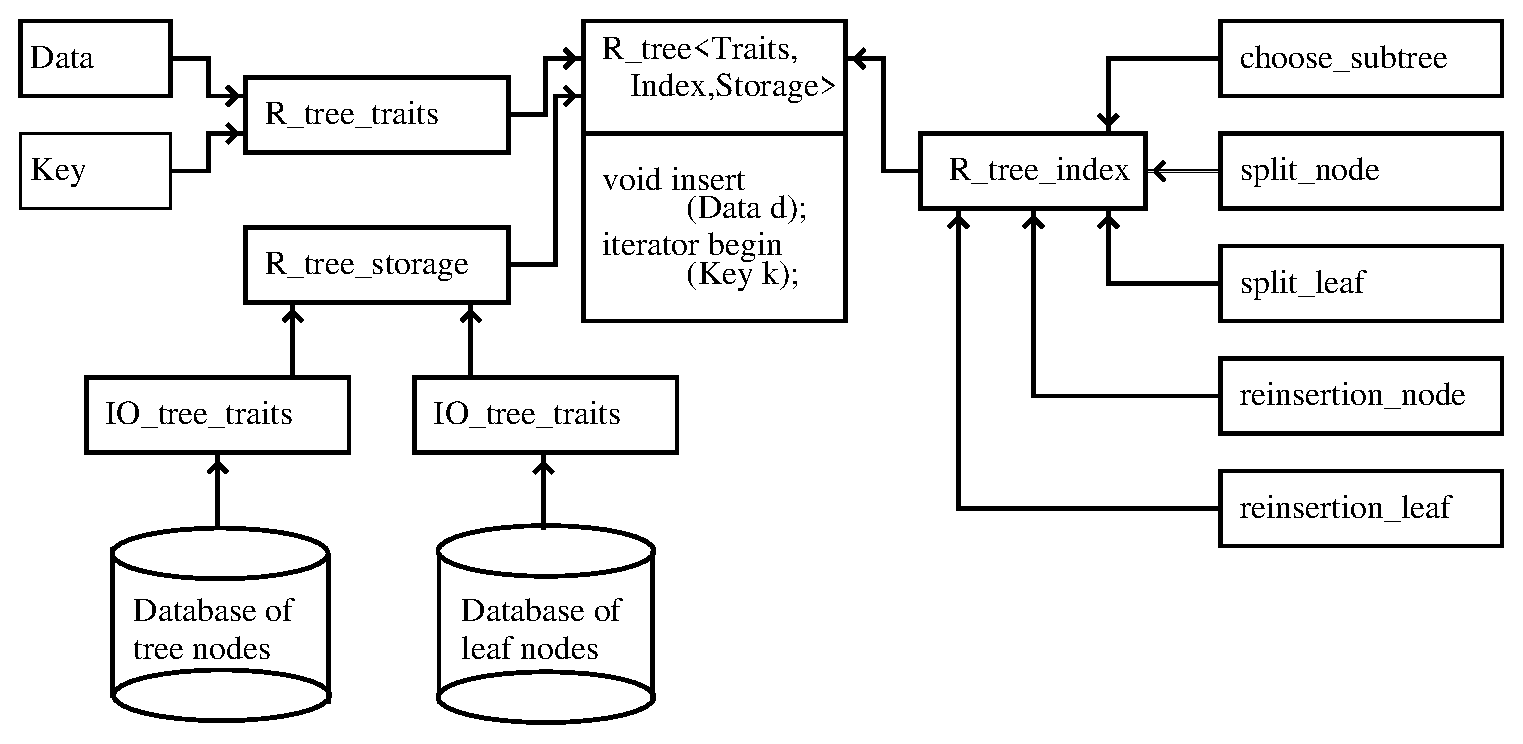
\includegraphics[width=14cm,clip]{rtree-classes4.eps}
\end{center}
\caption{\label{r-tree-design} R-Tree components}
\end{figure}
\end{ccTexOnly}
\begin{ccHtmlOnly}
    <!2><TABLE BORDER=0 CELLSPACING=2 CELLPADDING=0 WIDTH=650>
        <TR><TD ALIGN=LEFT VALIGN=TOP WIDTH=100% NOWRAP COLSPAN=2>
    <img border=0 src="./rtree-classes4.gif" alt="R-Tree components">
    </TD>
    <TD ALIGN=LEFT VALIGN=TOP WIDTH=50%><img border=0 src="./rtree-classes4.gif"
alt="R-Tree components">
      </TD></TR></TABLE>
\end{ccHtmlOnly}

\begin{ccTexOnly}
Figure~\ref{r-tree-design} shows the different components of the
R-Tree (R$^\star $-Tree) that can be plugged into the tree. 
\end{ccTexOnly}
\begin{ccHtmlOnly}
Figure~\ref{r-tree-design} shows the different components of the
R-Tree (R$^\star $-Tree) that can be plugged into the tree. 
\end{ccHtmlOnly}
The R-Tree has three template arguments. The \ccc{R-tree_traits}
class which defines the data handling, the \ccc{R_tree_index}
class which defines all \ccc{index} strategies and one traits
class which defines the databases and sizes of the tree nodes and
leaves. This class is called \ccc{R_tree_storage}. We now
describe each component more in detail. Note,
for
each component CGAL provides example classes or implementations
of the most important or most commonly used strategies.

\subsubsection{Data handling}
In this section we describe how data is handled in the tree.
\medskip

\noindent
{\bf Tree Data}\\
\noindent
The tree is designed to handle arbitrary spatial objects (called
\ccc{Data}) in arbitrary dimensions.
Each node of the tree stores a \ccc{Key} which usually is the
bounding box of the \ccc{Key}s of its childs. The tree is designed to be
independent of the form of a \ccc{Key}. 
That is a \ccc{Key} can have arbitrary dimension and arbitrary
form (e.g. a $d$-dimensional bounding box, the smallest enclosing
$d$-dimensional ball, etc). Nevertheless, the \ccc{Key} class has
to provide certain properties: 
E.g. for two \ccc{Key}s it must be decidable if one \ccc{Key} is contained in
the other one, if they intersect and what the smallest \ccc{Key}
is that encloses both \ccc{Key}s.
Besides access functions a \ccc{cost}-function has to be provided
that measures the inefficiency when clustering two \ccStyle{Key}s
together. This allows the user to build the R-Tree in respect to
different optimization functions such as minimum area, overlap or
margin enlargement when clustering two \ccStyle{Key}s together.
CGAL provides predefined
\ccc{Key} classes for $k$-dimensional aligned rectangles, $1\le k\le
4$ (see Section~\ref{k-key}). 
A traits class implementation that defines all necessary functions is
described in Section~\ref{interface}. 
\medskip

\noindent
{\bf R\_tree\_traits}\\
\noindent
The \ccc{Data}
and \ccc{Key} functionality is
accessed through a traits class we call \ccc{R_tree_traits}. This traits class decouples
the R-tree  from the \ccc{Data}
and \ccc{Key} class such that a modification of one of these classes
only affects this traits class but not the tree. 
The \ccc{R_tree_traits} class requirements are
described in  Section~\ref{interface}.
\cgal\ provides a predefined \ccc{R_tree_traits} class for the
predefined \ccc{Key} classes (see Section~\ref{Rtreetraitspre}). 
%The
%spatial objects are spatially clustered in the tree according to
%their orthogonal bounding boxes (called \ccStyle{Key}, see
%Section~\ref{k-key}).  A \ccStyle{Key} usually is a
%$k$-dimensional aligned rectangle, but it is also possible to
%define a different geometric object as \ccStyle{Key}. 



%The \ccc{cost}-function determines the cost of one key or the cost
%that arises when two keys are put together. The tree accesses the
%\ccc{cost}-function through a traits class and is therefore
%independent of the specific cost function.
%The user has to provide
%key specific functions that measure if two keys intersect,
%compute a penalty cost when clustering two keys together,
%etc. 

\subsubsection{R\_tree\_index}
The R-Tree index defines how the data is spatially clustered in
the tree. We decoupled the index strategies from the
implementation of the tree since many diffrent index
strategies have been proposed for the R-Tree. \cgal\ provides two 
\ccc{R_tree_index} classes that can be plugged into the tree: The
\ccc{R_tree_index} class which is the index strategy as
proposed by Guttman~\cite{gutt-84} and the \ccc{R_star_tree_index}
class which is the R$^\star$-Tree index strategy as proposed by  Beckmann
et al~\cite{Beckmann:1990:RER} (see Section~\ref{preindex}). The
requirements for a user defined \ccc{R_tree_index} class are
given in Section~\ref{indexreq}.
We here give a
short description of the index strategies.
\medskip

\noindent
{\bf choose\_subtree}\\
\noindent
In the \ccc{choose-subtree} strategy a subtree is chosen in which 
the new element is to be inserted. 
%Many \ccc{choose-subtree}
%strategies have been proposed. We therefore decoupled this
%strategy from the implementation of the R-Tree. 
We implemented
the \ccc{choose-subtree} strategy from Guttman~\cite{gutt-84}
and from Beckmann
et al~\cite{Beckmann:1990:RER} which can be plugged into the
tree (see Section~\ref{Choosepre}). The requirements for a user
defined \ccc{choose-subtree} strategy are given in
Section~\ref{userchoose}.
\medskip

\noindent
{\bf split\_node and split\_leaf}\\
\noindent
%Since many merging and splitting strategies have been proposed
%for the R-Tree and the R$^\star$-Tree we decoupled these strategies from the
%implementation of the R-Tree. 
The \ccc{split_node} and \ccc{split_leaf} method distributes the
entries of an overfilled inner node, resp. leaf, into two.
We implemented some important splitting
strategies like those from Guttman~\cite{gutt-84} and Beckmann
et al~\cite{Beckmann:1990:RER} which can be plugged into the
tree (see Section~\ref{Splitpre})
Note that one can plug in a different split strategy for the
inner nodes as for the leaf nodes of the tree.
See Section~\ref{userchoose} for the 
requirements a user implemented split strategy has to fulfill.
\medskip

\noindent
{\bf reinsertion\_node and reinsertion\_leaf}\\
\noindent
The R$^\star$-Tree forces entries to be reinserted during the
insertion routine. 
In the \ccc{reinsertion_node} and \ccc{reinsertion_leaf} method,
an overfilled node is divided into two parts. The one part stays
in that node and the other part is reinserted into the same level 
of the tree as the node is.
%Sine different reinsertion strategies have
%been proposed we decoupled these strategies from the
%implementation of the R-Tree. 
We implemented the
\ccc{close_reinsert} reinsertion
strategy of  Beckmann
et al~\cite{Beckmann:1990:RER} which can be plugged into the
tree. See Section~\ref{Reinsertpre} for the implementations of
the reinsertion strategies and  Section~\ref{userreinsert} for the
requirements a user implemented reinsertion strategy has to fulfill.
\medskip

\noindent
{\bf reinsertion}\\
\noindent
\label{reinsertion} 
The \ccc{R_tree_index} class gets a boolean template
  argument \ccc{reinsertion}. In case \ccc{reinsertion=true}
  entries are reinserted during the insertion process. More
  precisely, let a node be overfilled. Then, a part of the
  entries of this node is reinserted in case that no reinsertion 
  in the level of the node has been performed before. The entries 
  that are to be reinserted are chosen in the \ccc{reinsertion_node}
  class, \ccc{reinsertion_leaf} class, resp. Otherwise, a split is 
  performed. Note, the leaf level is the level number 0.

\subsubsection{R\_tree\_storage}
The \ccc{R_tree_storage} class  is a traits class in which all
storage dependant components of the R-Tree are defined. These are 
a database for the laef nodes, a database for the inner nodes of
the tree, the capacities of the nodes in form of the number of
elements and the size of a page, etc. \cgal\ provides two
predefined \ccc{R_tree_storage} classes called
\ccc{R_tree_internal_storage} and \ccc{R_tree_external_storage}
that can be plugged into the tree (see
Section~\ref{prestorage}). For the requirements of a user defined 
storage class see Section~\ref{storagereq}.
We now give a short description of the components of the
\ccc{R_tree_storage} class. 
\medskip

\noindent
{\bf Databases}\\
\noindent
The R-Tree has two databases. One for the inner nodes of the tree
and one for the leaf nodes. 

Each database is decoupled from the \ccc{R_tree_storage} class
 by an \ccc{IO_traits} 
class. %Both databases have to provide the same basic functionality. 
%We provide an I/O traits class that specifies the
%necessary functionality of a database (see Section~\ref{IOpre}). 
\cgal\ provides two databases for the R-Tree (see
Section~\ref{IOpre}). 
One stores the data and the tree in
internal memory. 
The other database  is an external memory database which
allocates a memory cache for $k$ pages of size pagesize, whereby $k$ is an
integer template argument. The cache uses the least recently used
strategy to load and unload pages. Note that other
databases  
can be plugged into the tree by providing an appropriate \ccc{IO_traits}
class. See Section~\ref{userIO} for the requirements a user
implemented database must fulfill.
\medskip

\noindent
{\bf Node and Leaf Capacities}\\
\noindent
The \ccc{R_tree_storage} class gets 4 integer template arguments.
The  minimum
capacity (\ccc{IO_min_cap_nodes}) and
maximum capacity (\ccc{IO_max_cap_nodes}) has to be defined for
an inner node of the tree.
Each inner node is guaranteed to have between \ccc{IO_min_cap_nodes} and
\ccc{IO_max_cap_nodes} \ccc{Key} entries; the root node has between 2 and
\ccc{IO_max_cap_nodes} entries. 
For the leaf nodes \ccc{IO_min_cap_leaves} defines the minimum
number of elements in a leaf and \ccc{IO_page_size} defines the maximum size of
all \ccc{Data} entries of a leaf.
\medskip

\noindent
{\bf headerextern}\\
\noindent
\ccc{headerextern} is a boolean template argument.
In case \ccc{header_extern=true}
  a header file containing necessary informations for the
  reconstruction of a tree from an external database is stored on
  disk. Otherwise, the header file is not stored on disk.

\subsubsection{More Features}
\begin{description}
\item[reinsertion control]
For each level of the tree, a reinsertion flag can be set to \ccc{true} 
or \ccc{false}. In case that the reinsertion flag of a level is
true, the \ccc{reinsertion_node} (\ccc{reinsertion_leaf} resp.)
routine will be called for an overfull node of this level (instead 
of the split routine). When the \ccc{reinsertion_node}
(\ccc{reinsertion_leaf} resp.) routine is finished, the
reinsertion flag is again set to \ccc{false} for that level.
See Section~\ref{r-tree} for a description 
of the functions \ccc{get_reinsertion_flag} and \ccc{set_reinsertion_flag}.
\item[output sensitive query function]
The query functions are output sensitive. That is, we
provide iterators that allow to intermix user code with
querying. Since the amount of query output can exceed
the main memory capacity there is no alternative than providing
output sensitive query functions (see Section~\ref{r-tree}).
\end{description}


%The implementation of the R-Tree follows the design issues of the
%generalized search tree~\cite{Hellerstein}. That is, the tree is designed
%to handle  arbitrary geometric objects (called \ccStyle{Data}) in
%arbitrary dimension. The traits class for the \ccc{Data} is
%described in  Section~\ref{data}. The
%spatial objects are spatially clustered in the tree according to
%their orthogonal bounding boxes (called \ccStyle{Key}, see
%Section~\ref{k-key}).  A \ccStyle{Key} usually is a
%$k$-dimensional aligned rectangle, but it is also possible to
%define a different geometric object as \ccStyle{Key}. CGAL provides predefined
%key classes for $k$-dimensional aligned rectangles, $1\le k\le
%4$. The user has to provide
%key specific functions that measure if two keys intersect,
%compute a penalty cost when clustering two keys together,
%etc. A traits class that defines all necessary functions is
%described in Section~\ref{interface}. This traits class is
%implemented out for the predefined key classes.
%The split strategies and the requirements for user
%defined split strategies are given in Section~\ref{split}.
%Since the split strategies work on predefined classes that
%contain either a key or a data element and some additional
%information on these elements, these classes are defined in Section~\ref{cont}.
%The definition of the \ccStyle{R_tree} is given in
%Section~\ref{r-tree}. In the end of this chapter an example is given.

%%%%%%%%%%%%%%%%%%%%%%%%%%%%%%%%%%%%%%%%%%%%%%%%%%%%%%%%%%%%%%%%%%%%%
%%%%%%%%%R-TREE%%%%%%%%%%%%%%%%%%%%%%%%%%%%%%%%%%%%%%%%%%%%%%%%%%%%%%
\section{R-Tree Class}
\label{r-tree}
\begin{ccClassTemplate}{R_tree<R_tree_traits, R_tree_index, R_tree_storage>}

\noindent
{\bf Class: R\_tree$<$R\_tree\_traits, R\_tree\_index, R\_tree\_storage$>$}

\ccDefinition
The R-Tree gets 3 template arguments.
\begin{description}
\item[\ccc{R_tree_traits}] This class builds the interface to the 
  \ccc{Data} and \ccc{Key}s of the tree. The requirements of this 
  class are defined in Section~\ref{treetraitsreq}. A predefined
  \ccc{R_tree_traits} class is described in
  Section~\ref{Rtreetraitspre}.
\item[\ccc{R_tree_index}] This class is a traits class in which
  the index strategies (\ccc{choose_subtree, split_node,
    split_leaf, reinsertion_node, reinsertion_leaf}) are
  defined. \cgal\ provides two predefined index traits classes
  (see Section~\ref{preindex}). The requirements for a user defined 
  index class are given in Section~\ref{indexreq}.
\item[\ccc{R_tree_storage}] This class is a traits class in which 
  the storage depending components are defined.  These are 
a database for the laef nodes, a database for the inner nodes of
the tree, the capacities of the nodes in form of the number of
elements and the size of a page, etc. \cgal\ provides two
predefined \ccc{R_tree_storage} classes called
\ccc{R_tree_internal_storage} and \ccc{R_tree_external_storage}
that can be plugged into the tree (see
Section~\ref{prestorage}). For the requirements of a user defined 
storage class see Section~\ref{storagereq}.
%\item[\ccc{Choose_subtree}] This class provides an \ccc{operator()} member
%function which gets all entries of a node, and a \ccc{Key} of
%a \ccc{Data} entrie that has to be inserted. It returns a node
%entrie that specifies the subtree in which the new \ccc{Data}
%entrie is to be inserted.  The requirements of this 
%  class are defined in Section~\ref{userchoose}. Predefined
%  \ccc{Choose_subtree} classes are described in Section~\ref{Choosepre}.
%\item[\ccc{Split_node}] An overfilled inner node of the tree is
%  split according to the split strategy that is defined in this
%  class. The requirements of this 
%  class are defined in Section~\ref{usersplit}. Predefined
%  \ccc{Split_node} classes are described in Section~\ref{Splitpre}.
%\item[\ccc{Split_leaf}] An overfilled leaf of the tree is
%  split according to the split strategy that is defined in this
%  class. The requirements of this 
%  class are defined in Section~\ref{usersplit}. Predefined
%  \ccc{Split_leaf} classes are described in Section~\ref{Splitpre}.
%\item[\ccc{Reinsertion_node}] In case that a part of an overfilled
%inner node is reinserted, the \ccc{reinsertion_node} strategy, which is
%defined in this class, is called. It computes the set of entries
%that is to be reinserted. The requirements of this 
%  class are defined in Section~\ref{userreinsert}. Predefined
%  \ccc{Reinsertion_node} classes are described in
%  Section~\ref{Reinsertpre}.
%\item[\ccc{Reinsertion_leaf}] In case that a part of an overfilled
%inner leaf is reinserted, the \ccc{reinsertion_leaf} strategy, which is
%defined in this class, is called. It computes the set of entries
%that is to be reinserted. The requirements of this 
%  class are defined in Section~\ref{userreinsert}. Predefined
%  \ccc{Reinsertion_leaf} classes are described in Section~\ref{Reinsertpre}.
%\item[\ccc{IO_tree_traits_nodes}] This class specifies the
%  database for the inner nodes of the tree. The requirements of this 
%  class are defined in Section~\ref{userIO}. Predefined
%  \ccc{IO_tree_traits_node} classes are described in
%  Section~\ref{IOpre}.
%\item[\ccc{IO_tree_traits_leaf}] This class specifies the
%  database for the leaf nodes of the tree. The requirements of this 
%  class are defined in Section~\ref{userIO}. Predefined
%  \ccc{IO_tree_traits_leaf} classes are described in Section~\ref{IOpre}.
%\item[\ccc{IO_pagesize}] This integer template argument specifies 
%  the size of a page. The tree and leaf data is stored in disk
%  blocks of this size.
%This size must be smaller than a third of the
%  size of the
%  internal memory such that at least three pages can be kept in
%  internal memory without swapping.
%\item[\ccc{header_extern}] The R-Tree gets a boolean template
%  argument \ccc{header_extern}. In case \ccc{header_extern=true}
%  a header file containing necessary informations for the
%  reconstruction of a tree from an external database is stored on
%  disk. Otherwise the header file is not stored on disk.
\end{description}
\ccInclude{CGAL/R_tree.h}


\ccCreationVariable{R}


\ccCreation
\ccConstructor{R_tree();}{An empty R-Tree is constructed.}
\ccConstructor{R_tree(char *header_file, char *node_data_file,
  char *leaf_data_file);}{An R-Tree is initialized. In case that
  the \ccc{header_file} is not empty, the tree expects that
  \ccc{header_file}, \ccc{node_data_file} and
  \ccc{leaf_data_file} are files that were generated by the same
  type of R-Tree as this type is. That is, all template classes
  have to be identic. Furthermore, the files must belong
  together. In this case, the tree is build according to the data 
  in the files. Otherwise, if \ccc{header_file} is an empty file, 
  an empty tree is constructed.}

\ccOperations

%\ccMethod{void ~R_tree();}{The R-Tree is destructed. The databases are 
%  closed.}

%\ccMethod{void open(char *header_file, char *node_data_file,
%  char *leaf_data_file);}{An R-Tree is initialized. In case that
%  the \ccc{header_file} is not empty, the tree expects that
%  \ccc{header_file}, \ccc{node_data_file} and
%  \ccc{leaf_data_file} are files that were generated by the same
%  type of R-Tree as this type is. That is, all template classes
%  have to be identic. Furthermore, the files must belong
%  together. In this case, the tree is build according to the data 
%  in the files. Otherwise, if \ccc{header_file} is an empty file, 
% an empty tree is constructed.}

\ccMethod{void insert(Data& elem);}{A new element is inserted into 
  the tree.}

\ccMethod{bool find_key_include(Key a);}{If the tree contains a
  \ccc{Data} element that is contained in \ccc{Key a}, then \ccc{true} is
  returned. Otherwise, \ccc{false} is returned.}

\ccMethod{bool find_key_intersect(Key a);}{If the tree contains a
  \ccc{Data} element with a \ccc{Key k} that has non empty
  intersection with \ccc{Key a}, then \ccc{true} is
  returned. Otherwise, \ccc{false} is returned.}

\ccMethod{bool delete_key(Key& a, Data& elem);}{If the tree
  contains a \ccc{Data} element with \ccc{Key a}, then \ccc{elem} is
  set to this \ccc{Data} element and true is returned. Otherwise, 
  false is returned. Note, only one \ccc{Data} element with
  \ccc{Key a} is deleted. In order to delete another element with
  \ccc{Key a} you have to repeat the function call.}

\ccMethod{int get_rootlevel();}{The level of the root is returned.}

\ccMethod{bool get_reinsertion_flag(int the_level);}{The
  reinsertion flag of \ccc{the_level} is returned.}

\ccMethod{bool set_reinsertion_level(unsigned int the_level,bool
  value);}{The reinsertion flag of level \ccc{the_level} is set
  to \ccc{value}. If \ccc{value=true} then a part of an overfilled node in
  level \ccc{the_level} will be reinserted.}

\ccMethod{void dump();}{The tree is dumped in a readable way to \ccc{stderr}.}


\ccMethod{R_tree::iterator begin_intersect();}{An forward
  iterator that iterates through all \ccc{Data} elements of the
  tree is initialized and returned. In
  order to iterate through all elements of the tree you should
  compare your actual iterator with the \ccc{end_intersect()}
  iterator. If both iterators are identical, you reached past the
  last 
  element.}

\ccMethod{R_tree::iterator end_intersect();}{An forward
  iterator that iterates through all \ccc{Data} elements of the
  tree is initialized with the last element and returned. In
  order to iterate through all elements of the tree you should
  compare your actual iterator with the \ccc{end_intersect()}
  iterator. If both iterators are identical, you reached past the last 
  element.}

\ccMethod{R_tree::iterator begin_intersect(Key k);}{An forward
  iterator that iterates through all \ccc{Data} elements of the
  tree that have non empty intersection with \ccc{Key k} is
  initialized 
  and returned. In
  order to iterate through all elements of the tree  that have
  non empty intersection with \ccc{Key k}  you should
  compare your actual iterator with the \ccc{end_intersect(k)}
  iterator. If both iterators are identical, you reached past the last 
  element.}

\ccMethod{R_tree::iterator end_intersect(Key k);}{An forward
  iterator that iterates through all \ccc{Data} elements of the
  tree that have non empty intersection with \ccc{Key k} is
  initialized  with the last element and returned. In
  order to iterate through all elements of the tree that have non 
  empty intersection with \ccc{Key k} you should
  compare your actual iterator with the \ccc{end_intersect(k)}
  iterator. If both iterators are identical, you reached past the last 
  element.}

\ccMethod{R_tree::iterator begin_enclose(Key k);}{An forward
  iterator that iterates through all \ccc{Data} elements of the
  tree that enclose \ccc{Key k} is
  initialized 
  and returned. In
  order to iterate through all elements of the tree  that enclose
  \ccc{Key k}  you should
  compare your actual iterator with the \ccc{end_enclose(k)}
  iterator. If both iterators are identical, you reached past the last 
  element.}

\ccMethod{R_tree::iterator end_enclose(Key k);}{An forward
  iterator that iterates through all \ccc{Data} elements of the
  tree that enclose \ccc{Key k} is
  initialized  with the last element and returned. In
  order to iterate through all elements of the tree that enclose
   \ccc{Key k} you should
  compare your actual iterator with the \ccc{end_enclose(k)}
  iterator. If both iterators are identical, you reached past the last 
  element.}

\ccMethod{R_tree::iterator begin_compare(Key k);}{An forward
  iterator is initialized and returned. It iterates through all 
  \ccc{Data} elements $a$ of the
  tree for which \ccc{R_tree_traits::compare(Key k,a)=true}
  and for all \ccc{p(a)} \ccc{R_tree_traits::compare(Key k,p(a))=true},
  whereby \ccc{p(a)} is a key of an ancestor of \ccc{a} in the
  tree. In 
  order to iterate through all elements of the tree  that compare 
  with 
  \ccc{Key k}  you should
  compare your actual iterator with the \ccc{end_compare(k)}
  iterator. If both iterators are identical, you reached past the last 
  element. Note that the \ccc{compare} function is no where else used in
  the tree than for this search. Therefore, you can freely define 
  what kind of comparison is to be done.}

\ccMethod{R_tree::iterator end_compare(Key k);}{An forward
  iterator  is
  initialized  with the last element and returned.
It iterates through all 
  \ccc{Data} elements $a$ of the
  tree for which \ccc{R_tree_traits::compare(Key k,a)=true}
  and \ccc{R_tree_traits::compare(Key k,p(a))=true},
  whereby \ccc{p(a)} is a key of an ancestor of \ccc{a} in the
  tree.
  In order to iterate through all elements of the tree that
  compare with
   \ccc{Key k} you should
  compare your actual iterator with the \ccc{end_compare(k)}
  iterator. If both iterators are identical, you reached past the last 
  element.
Note that the \ccc{compare} function is no where else used in
  the tree than for this search. Therefore, you can freely define 
  what kind of comparison is to be done.}

\end{ccClassTemplate}

\begin{ccClass}{R_tree::iterator }

\noindent
{\bf Class: R\_tree::iterator}

\ccDefinition
Defines an iterator over R-Tree \ccc{Data} objects.

\ccCreationVariable{I}


\ccCreation

\ccConstructor{R_tree::iterator();}{}


\ccOperations

\ccMethod{bool operator==(R_tree::iterator & x);}{Let the
  iterators point on the \ccc{Data} elements \ccc{a} and \ccc{b}. 
  Then, \ccc{R_tree_traits::equal_data(a,b)} is returned.}
\ccMethod{bool operator!=(R_tree::iterator& x);}{Let the
  iterators point on the \ccc{Data} elements \ccc{a} and \ccc{b}. 
  Then, \ccc{!R_tree_traits::equal_data(a,b)} is returned.}
\ccMethod{R_tree::iterator& operator=(R_tree::iterator x);}{The
  iterator is set to iterator \ccc{x}.}
\ccMethod{Data operator*();}{The \ccc{Data} element the iterator
  points to is returned.}
\ccMethod{bool is_valid();}{Returns \ccc{true}, if the iterator
  points on a valid \ccc{Data} element.}
\ccMethod{R_tree::iterator& operator++();}{Depending on the query 
  function (intersection, enclose, compare), the iterator is moved
  to the next element that matches the query in respect to the 
  \ccc{Key} the iterator was initialized with.}
\ccMethod{void operator++(int );}{Same as calling \ccc{operator++()}.}

\end{ccClass}


%%%%%%%%%%%%%%%%%%%%%%%%%%%%%%%%%%%%%%%%%%%%%%%%%%%%%%%%%%%%%%%%%%%%%
%%%%%%%%%%%%%%%%%%%%%%%%%%%%%%%%%%%%%%%%%%%%%%%%%%%%%%%%%%%%%%%%%%%%%
%%%%%%%%%%%%%%%% Predefined Keys   %%%%%%%%%%%%%%%%%%%%%%%%%%%%%%%%%%
\section{R-Tree Traits Class Implementations for Data handling}
In this section we describe all predefined classes for the Data
handling, that can be
plugged into the R-Tree.
\subsection{Predefined $k$-dimensional Keys}
\label{k-key}
\cgal\ provides four key classes for $k\in\{1,\ldots,4\}$.
%\begin{ccClassName}{R\_tree\_key\_\tt k\ccFont }
\begin{ccClass}{R_tree_key_k}

\noindent
{\bf Class: R\_tree\_key\_k}

\ccDefinition

An object of the class  \ccClassName\ is a $k$-dimensional iso rectangle.

\ccInclude{CGAL/R_tree_key.h}


\ccCreationVariable{K}


\ccCreation

\ccConstructor{R_tree_key_k ();}{Introduces a $k$-dimensional aligned rectangle.}



\ccConstructor{R_tree_key_k(int x1_min, int
  x1_max,..., int xk _min, int xk _max );}{Introduces a $k$-dimensional aligned rectangle initialized with \ccc{int x1_min, int
  x1_max,..., int xk _min, int xk _max }.}



\ccOperations

\ccMethod{bool operator==(R_tree_key_kt a);}{
Returns true if \ccc{K} is equal to \ccc{a}.}

%\ccMethod{R_tree_key_k operator=(R_tree_key_kFont a);}{
\ccMethod{R_tree_key_k operator=(R_tree_key_k a);}{
Sets \ccc{K} to  \ccc{a}.}

\ccMethod{double cost();}{
Depending on the dimension $k$ the interval length, area, or volume is returned.}


\ccMethod{void unify(R_tree_key_k a,
  R_tree_key_k b);}
{\ccc{K} is set to bounding box of \ccc{a} $\cup $\ccc{b}.}

\ccMethod{bool include(R_tree_key_k a);}
{Returns true if \ccc{K} includes \ccc{a}.}

\ccMethod{bool intersect(R_tree_key_k a);}
{Returns true if \ccc{K} and \ccc{a} intersect.}

\ccMethod{void intersection(R_tree_key_k a,
  R_tree_key_k b);}
{\ccc{K} is set to  \ccc{a} $\cap$ \ccc{b}. This method is only
  necessary when the R$^\star$-Tree split strategy of Beckman et
  al~\cite{Beckmann:1990:RER} is plugged into the tree (see
  Section~\ref{Splitpre}).}

\ccMethod{double center\_dist(R_tree_key_k a);}
{Computes the center point of \ccc{K} and  \ccc{a} and returns
  the squared Euclidean distance between their center points. 
This method is only
  necessary when the R$^\star$-Tree reinsertion strategy of Beckman et
  al~\cite{Beckmann:1990:RER} is plugged into the tree (see
  Section~\ref{Splitpre}).}


\ccMethod{void write(fstream& s);}
{Writes \ccc{*this} to s.}

\ccMethod{void read(fstream& s);}
{Reads \ccc{*this} from s.}

\ccMethod{void dump(int depth=0);}
{Writes \ccc{*this} in a readable way to \ccc{stderr}.}

\end{ccClass}

%%%%%%%%%%%%%%%%%%%%%%%%%%%%%%%%%%%%%%%%%%%%%%%%%%%%%%%%%%%%%%%%%%%%%
\subsection{Predefined Sort\_axis Classes for the $k$-dimensional Keys}
\label{Presort}
\cgal\ provides four \ccc{Sort_axis} classes, one for each
predefined $k$-dimensional Key, $k\in\{1,\ldots,4\}$. In fact,
these classes also work on user defined $k$-dimensional \ccc{Key} classes that
provide $k$ function objects \ccc{compare_1,\dots ,compare_k}
each taking two \ccc{Keys} as argument and returning \ccc{true}
if the minimum coordinate of the first argument is leftmost.   Each class
has an \ccc{bool operator()(int
  split_axis, Container *first, Container *last)} which sorts the
sequence \ccc{[first,last[} according to their \ccc{Key}s and the
\ccc{split_axis}. In
case that \ccc{split_axis} is greater equal than the dimension of
the \ccc{Key}, \ccc{false} is returned. Otherwise, true is returned.
This class is needed  as a template argument for the
implementation of the split strategies of  Beckmann
et.al.~\cite{Beckmann:1990:RER} (see Section~\ref{Splitpre}). 


\begin{ccClassTemplate}{sort_axis_key_k_dim<Container>}

\noindent
{\bf Class: sort\_axis\_key\_{\tt k}\_dim$<$Container$>$}\\
\noindent
\ccDefinition

The class \ccc{Container} defines the type \ccc{Key}. It has a
member of type \ccc{Key} which is called \ccc{key}. 

\ccInclude{CGAL/R_tree_key.h}

\ccCreationVariable{S}


\ccCreation

\ccOperations
\ccMethod{bool operator()(int sort_axis, Container *first,
  Container *last);}{If the number \ccc{sort_axis} is smaller
  than the dimension of the \ccc{Container::Key}, then, the
  entries \ccc{[first,last]} are sorted according to the
  \ccc{sort_axis}-1 th axis and \ccc{true} is returned.
  The sorting is processed by calling
  the STL \ccc{stable_sort} function. If the number
  \ccc{sort_axis} is greater than  or equal to
   the dimension of the \ccc{Container::Key}, then false is
   returned.\\
  \ccc{Precondition:} the $k$-dimensional \ccc{Key} class
provides $k$ function objects \ccc{compare_1,\dots ,compare_k}
each taking two \ccc{Keys} as argument and returning \ccc{true}
if the minimum coordinate of the first argument is leftmost.}
\end{ccClassTemplate}


%%%%%%%%%%%%%%%%%%%%%%%%%%%%%%%%%%%%%%%%%%%%%%%%%%%%%%%%%%%%%%%%%%%%%
\subsection{Predefined R\_tree\_traits Class}
\label{Rtreetraitspre}
\begin{ccClassTemplate}{R_tree_traits<R_tree_data>}
\noindent
{\bf Class: R\_tree\_traits$<$R\_tree\_data$>$}

\cgal\  provides a predefined \ccc{R_tree_traits} for \ccc{Data}
classes that have a predefined \ccc{Key} class as
member. Furthermore, the \ccc{Data} class has to provide a \ccc{read}
and a \ccc{write} function.
This traits class is  the interface to the \ccc{Data} and the 
\ccc{Key} of the \ccc{R_tree} class. Therefore, the tree is
independent of the \ccc{Data} and 
\ccc{Key} class. The \ccc{Data} and 
\ccc{Key} elements are only accessed through this traits
class. This has the advantage that a change of the \ccc{Data} or 
\ccc{Key} class has only impact on the traits class but not on
the tree. Furthermore, the traits class allows to plug in  arbitrary Data e.g. 
a \ccc{CGAL::Polygon_2} or a
\ccc{CGAL::Segment_2}. 
Two methods are only necessary, when  R$^\star$-Tree
split methods or reinsertion methods are plugged into the
tree. These methods are highlighted.



\ccInclude{CGAL/R_tree_traits.h}


\ccCreationVariable{T}

\ccTypes
\ccTypedef{typedef R_tree_traits Traits;}{}
\ccTypedef{typedef R_tree_data::Key Key;}{}
\ccTypedef{typedef R_tree_data Data;}{}


\ccCreation

\ccConstructor{R_tree_traits();}
{Introduces a tree traits.}

\ccOperations

\ccMethod{ size_t size(Data d);}
{Returns the size of \ccc{d}. 
\ccPrecond \ccc{Data} has a member function \ccc{size_t size();}}

\ccMethod{Key build(Data &d);}
{Returns the key of \ccc{d}.}

\ccMethod{double cost(Key a);}
{Returns the \ccc{cost} of \ccc{a}.}

\ccMethod{double cost(Key a, Key b);}
{Returns the \ccc{cost} of \ccc{a}$\cup$\ccc{b}. According to
  Guttman, here the inefficiency cost of clustering \ccc{a} with
  \ccc{b} together
  should returned. More precisely,
  \ccc{cost(unify(a,b))-cost(a)-cost(b)} is returned.}


\ccMethod{Key unify(Key  a, Key b);}
{Returns the bounding box of \ccc{a} $\cup $\ccc{b}.}

\ccMethod{bool include(Key a, Key b);}
{Returns true if \ccc{a} includes \ccc{b}.}

\ccMethod{bool intersect(Key a, Key b);}
{Returns true if \ccc{a}  and \ccc{b} intersect.}

\ccMethod{Key intersection(Key a, Key b);}
{\ccc{K} is set to  \ccc{a} $\cap$ \ccc{b}. This method is only
  necessary when the R$^\star$-Tree split strategy of Beckman et
  al~\cite{Beckmann:1990:RER} is plugged into the tree (see
  Section~\ref{Splitpre}).}

\ccMethod{double center_dist(Key a, Key b);}{
Computes the center point of \ccc{K} and  \ccc{a} and returns
  the squared Euclidean distance between their center points. 
This method is only
  necessary when the R$^\star$-Tree reinsertion strategy of Beckman et
  al~\cite{Beckmann:1990:RER} is plugged into the tree (see
  Section~\ref{Splitpre}).}

\ccMethod{void read(char *s, Data a);}
{\ccc{a} is initialized with \ccc{s}.
\ccPrecond \ccc{Data} has a member function \ccc{void read(char *s);}}

\ccMethod{void write(char *s, Data a);}
{\ccc{a} is written to \ccc{s}. \ccc{s} has size \ccc{size(a)}.
\ccPrecond \ccc{Data} has a member function \ccc{void write(char *s);}}

\ccMethod{void dump(int depth=0);}
{Writes the data or the key in a readable way to \ccc{stderr}.}

\end{ccClassTemplate}


%%%%%%%%%%%%%%%%%%%%%%%%%%%%%%%%%%%%%%%%%%%%%%%%%%%%%%%%%%%%%%%%%%%%
\section{R-Tree Traits Class Implementations for the R-Tree
  Index}
In this section we describe the predefined \ccc{R_tree_index}
classes and their components.

\subsection{Predefined R-Tree Index classes}
\label{preindex}
The \ccc{R_tree} class gets a \ccc{R_tree_index} class as
template argument. This class defines all index strategies of the 
tree. These strategies  define how the data is spatially clustered in
the tree.
\subsubsection{Predefined R-Tree Index Class}
Predefined index class that contains the index strategies of the
R-Tree of Guttmann~\cite{gutt-84}.
\begin{ccClassTemplate}{R_tree_index<R_tree_traits>}

\noindent
{\bf Class: R\_tree\_index$<$R\_tree\_traits$>$}

\ccDefinition
\ccInclude{CGAL/R_tree_index.h}

\ccTypes

\ccTypedef{typedef choose_subtree<R_tree_value<
    R_tree_traits>, R_tree_traits>
    Choose_subtree;}{Defines the choose subtree strategy (see Section~\ref{Choosepre}).}
\ccTypedef{typedef quadratic_split_node<R_tree_value<
     R_tree_traits>, R_tree_traits>
    Split_node;}{Defines the split strategy for the inner nodes
    of the tree (see Section~\ref{Splitpre}).}
\ccTypedef{typedef quadratic_split_leaf<R_tree_leaf_data<
    R_tree_traits>, R_tree_traits>
    Split_leaf;}{Defines the split strategy for the leaves
    of the tree (see Section~\ref{Splitpre}).}
\ccTypedef{typedef dummy_reinsertion_node<R_tree_value<
    R_tree_traits>, R_tree_traits>
    Reinsertion_node;}{Defines the reinsertion node strategy (see
    Section~\ref{Reinsertionpre}).}
\ccTypedef{typedef dummy_reinsertion_leaf<R_tree_leaf_data<
    R_tree_traits>, R_tree_traits>
    Reinsertion_leaf;}{Defines the reinsertion leaf strategy (see
    Section~\ref{Reinsertionpre}).}
%\ccMembers
\ccTypedef{const static bool reinsertions=false;}{Reinsertions
  are prohibited}

\end{ccClassTemplate}

\subsubsection{Predefined R$^\star$-Tree Index Class}
Predefined index class that contains the index strategies of the
R$^\star$-tree of Beckmann et al~\cite{Beckmann:1990:RER}.
\begin{ccClassTemplate}{R_star_tree_index<R_tree_traits>}

\noindent
{\bf Class: R\_star\_tree\_index$<$R\_tree\_traits$>$}

\ccDefinition
\ccInclude{CGAL/R_star_tree_index.h}

\ccTypes

\ccTypedef{typedef star_choose_subtree<R_tree_value<
    R_tree_traits>, R_tree_traits>
    Choose_subtree;}{Defines the choose subtree strategy (see Section~\ref{Choosepre}).}
\ccTypedef{typedef star_split_node<R_tree_value<
     R_tree_traits>, R_tree_traits,
    sort_axis_key_2_dim<R_tree_value<R_tree_traits> > >
    Split_node;}{Defines the split strategy for the inner nodes
    of the tree (see Section~\ref{Splitpre}).}
\ccTypedef{typedef star_split_leaf<R_tree_leaf_data<
    R_tree_traits>, R_tree_traits, sort_axis_key_2_dim<R_tree_leaf_data<R_tree_traits> > >
    Split_leaf;}{Defines the split strategy for the leaves
    of the tree (see Section~\ref{Splitpre}).}
\ccTypedef{typedef reinsertion_node<R_tree_value<
    R_tree_traits>, R_tree_traits>
    Reinsertion_node;}{Defines the reinsertion node strategy (see
    Section~\ref{Reinsertionpre}).}
\ccTypedef{typedef reinsertion_leaf<R_tree_leaf_data<
    R_tree_traits>, R_tree_traits>
    Reinsertion_leaf;}{Defines the reinsertion leaf strategy (see Section~\ref{Reinsertionpre}).}
%\ccMembers
\ccTypedef{const static bool reinsertions=true;}{Do reinsertions.}
\end{ccClassTemplate}



\subsection{Predefined R-Tree Choose Subtree Strategies}
\label{Choosepre}

The \ccc{R_tree_index} class gets a \ccc{choose_subtree} class as template
argument. For a sequence container of node entries and a
\ccc{Key} $k$ of a \ccc{Data} element that has to be inserted
into the tree, a node entrie  is determined and returned. This
node entrie specifies the subtree in which the \ccc{Data}
element will be inserted.
\cgal\  provides the \ccc{choose_subtree}
strategy of Guttman~\cite{gutt-84} and the
\ccc{star_choose_subtree} 
strategy of Beckmann
et.al.~\cite{Beckmann:1990:RER}. 

\subsubsection{Guttman's Choose Subtree Strategy}

\begin{ccClassTemplate}{choose_subtree<Container,R_tree_traits>}

\noindent
{\bf Class: choose\_subtree$<$Container, R\_tree\_traits$>$}

\ccDefinition
The \ccc{Container} has a member
\ccc{key} which is of
type \ccc{Key} and contains the key of the subtree.
The choose subtree method works
on this class. 
See Section~\ref{Rtreetraitspre} and~\ref{treetraitsreq} for the definition and member
functions of class \ccc{R_tree_traits}.

\ccInclude{CGAL/R_tree_index_implementations.h}
\ccCreationVariable{s}

\ccCreation
\ccConstructor{choose_subtree();}{}

\ccOperations

\ccMethod{Container *operator()(Key k, Container *first,
  Container *last, int level);}{
For each entry in the sequence container \ccc{[first,last]} the
area enlargement to include the new \ccc{Key k} is computed. The
\ccc{Container} element with the smallest area enlargement is
returned. Ties are resolved by choosing the element of smallest area.}

\end{ccClassTemplate}

\subsubsection{R$^\star$-Tree Choose Subtree Strategy}

\begin{ccClassTemplate}{star_choose_subtree<Container,R_tree_traits>}

\noindent
{\bf Class: star\_choose\_subtree$<$Container,R\_tree\_traits$>$}

\ccDefinition
The \ccc{Container} has a member
\ccc{key} which is of
type \ccc{Key} and contains the key of the subtree.
The choose subtree method works
on this class. 
See Section~\ref{Rtreetraitspre} and~\ref{treetraitsreq} for the definition and member
functions of class \ccc{R_tree_traits}.

\ccInclude{CGAL/R_tree_index_implementations.h}
\ccCreationVariable{s}

\ccCreation
\ccConstructor{star_choose_subtree();}{}

\ccOperations
\ccMethod{Container *operator()(Key k, Container *first,
  Container *last, int level);}{
If \ccc{level} is the first level of the tree (the leaves are on
level 0), then
for each entry in the sequence container \ccc{[first,last]} the
overlap enlargement to include the new \ccc{Key k} is computed. The
\ccc{Container} element with the smallest area enlargement is
returned. Ties are resolved by choosing the element with smallest
area enlargement.
Otherwise, for each entry in the sequence container \ccc{[first,last]} the
area enlargement to include the new \ccc{Key k} is computed. The
\ccc{Container} element with the smallest area enlargement is
returned. Ties are resolved by choosing the element of smallest area.} 

\end{ccClassTemplate}


%\section{Predefined R-Tree Traits Classes}

%%%%%%%%%%%%%%%% Split strategies   %%%%%%%%%%%%%%%%%%%%%%%%%%%%%%%%%%
\subsection{Predefined R\_tree Split Strategies}
\label{split}
\label{Splitpre}
The \ccc{R_tree_index} gets two split classes as template
arguments. One splits an inner vertex of the tree and
one a leaf of the tree. \cgal\  provides the quadratic split
strategy from Guttman~\cite{gutt-84}. 
Furthermore \cgal\  provides an 
implementation of the split strategy of Beckmann
et.al.~\cite{Beckmann:1990:RER}. 

\subsubsection{Guttman quadratic split}

\begin{ccClassTemplate}{quadratic_split_leaf<Container,R_tree_traits>}

\noindent
{\bf Class: quadratic\_split\_leaf$<$Container,R\_tree\_traits$>$}

%\begin{ccClassName}{quadratic\_split}
\ccDefinition

The \ccc{Container} has two members: \ccc{ele} is of
type \ccc{Data} and contains a data element, and \ccc{key} is of
type \ccc{Key} and contains the key of the data element.
The split operation works
on this class. 
See Section~\ref{Rtreetraitspre} and~\ref{treetraitsreq} for the definition and member
functions of class \ccc{R_tree_traits}.

\ccInclude{CGAL/R_tree_index_implementations.h}
\ccCreationVariable{s}
\ccCreation
\ccConstructor{quadratic_split_leaf();}{}


\ccOperations
\ccMethod{void operator()(Container *first, Container *last, 
                back_insert_iterator<vector<Container *> > left,  
                back_insert_iterator<vector<Container *> > right,
                unsigned int minEntries, unsigned int pagesize);}
{The \ccc{Container} elements in \ccc{[first, last]} are
  subdivided into two vectors: \ccc{left} and
  \ccc{right}. Firstly, the two data elements \ccc{a} and \ccc{b}
  in \ccc{[first,
    last]} are computed with \ccc{R_tree_traits.cost(a,b)} is
  maximum. \ccc{a} is put into vector \ccc{right} and \ccc{b} is
  put into vector \ccc{left}. As long as not all elements in
  \ccc{[first, last]} are put into a vector, the element \ccc{c} with 
\ccc{R_tree_traits.cost(a,c)} or \ccc{R_tree_traits.cost(b,c)} is
  minimum is determined and put into the corresponding vector. It
  is made sure that each vector contains at least
  \ccc{minEntries} elements and all \ccc{Data} elements of each
  vector have size 
  at most \ccc{pagesize}.}

\end{ccClassTemplate}

\begin{ccClassTemplate}{quadratic_split_node<Container, R_tree_traits>}
%\begin{ccClassName}{quadratic\_split\_node}

\noindent
{\bf Class: quadratic\_split\_node$<$Container, R\_tree\_traits$>$}

\ccDefinition
The \ccc{Container} has a member
\ccc{key} which is of
type \ccc{Key} and contains the key of the subtree.
The split operation works
on this class. 
See Section~\ref{Rtreetraitspre} and~\ref{treetraitsreq} for the definition and member
functions of class \ccc{R_tree_traits}.

\ccInclude{CGAL/R_tree_index_implementations.h}
\ccCreationVariable{s}

\ccCreation
\ccConstructor{quadratic_split_node();}{}


\ccOperations
\ccMethod{void operator()(Container *first, Container *last, 
                  Container *left, Container *right,
                  int minEntries, int maxEntries);}{
The \ccc{Container} elements in \ccc{[first, last]} are
  subdivided into two sequence containers: \ccc{left} and
  \ccc{right}. Firstly, the two  elements \ccc{a} and \ccc{b}
  in \ccc{[first,
    last]} are computed with \ccc{R_tree_traits.cost(a,b)} is
  maximum. \ccc{a} is put into  \ccc{right} and \ccc{b} is
  put into  \ccc{left}. As long as not all elements in
  \ccc{[first, last]} are put into a sequence container, the element \ccc{c} with 
\ccc{R_tree_traits.cost(a,c)} or \ccc{R_tree_traits.cost(b,c)} is
  minimum is determined and put into the corresponding sequence
  container. It is made sure that each sequence container
  \ccc{left} and \ccc{right} contains between \ccc{minEntries} and
  \ccc{maxEntries} entries.
}

\end{ccClassTemplate}



%\subsubsection{Modified Guttman quadratic split
%  (linear\_split\_leaf, linear\_split\_node)}
%
%\begin{ccClassTemplate}{linear_split_leaf<Container,R_tree_traits>}
%
%\noindent
%{\bf Class: linear\_split\_leaf$<$Container,R\_tree\_traits$>$}
%
%%\begin{ccClassName}{quadratic\_split}
%\ccDefinition
%
%The \ccc{Container} has two members: \ccc{ele} is of
%type \ccc{Data} and contains a data element, and \ccc{key} is of
%type \ccc{Key} and contains the key of the data element.
%The split operation works
%on this class. See Section~\ref{Rtreetraitspre} and~\ref{treetraitsreq} for the definition and member
%functions of class \ccc{R_tree_traits}.
%
%\ccInclude{CGAL/R_tree_split.h}
%\ccCreationVariable{s}
%
%
%\ccCreation
%\ccConstructor{linear_split_leaf();}{}
%
%\ccOperations
%\ccMethod{void operator()(Container *first, Container *last, 
%                back_insert_iterator<vector<Container *> > left,  
%                back_insert_iterator<vector<Container *> > right,
%                unsigned int minEntries, unsigned int
%                pagesize);}{
%The \ccc{Container} elements in \ccc{[first, last]} are
%  subdivided into two vectors: \ccc{left} and
%  \ccc{right}. Firstly, the two \ccc{Data} elements \ccc{a} and \ccc{b}
%  in \ccc{[first,
%    last]} are computed with \ccc{R_tree_traits.cost(a,b)} is
%  maximum. \ccc{a} is put into vector \ccc{right} and \ccc{b} is
%  put into vector \ccc{left}. After that, the rest of the
%  elements in
%  \ccc{[first, last]} are put into that vector for which the
%  the insertion of the element produces a minimum cost. It
%  is made sure that each vector contains at least
%  \ccc{minEntries} elements and the \ccc{Data} elements have size 
%  at most \ccc{pagesize}.}
%
%\end{ccClassTemplate}
%
%
%\begin{ccClassTemplate}{linear_split_node<Container,
%    R_tree_traits>}
%
%\noindent
%{\bf Class: linear\_split\_node$<$Container,R\_tree\_traits$>$}
%%\begin{ccClassName}{quadratic\_split\_node}
%
%
%\ccDefinition
%The \ccc{Container} has a member
%\ccc{key} which is of
%type \ccc{Key} and contains the key of the subtree.
%The split operation works
%on this class. 
%See Section~\ref{Rtreetraitspre} and~\ref{treetraitsreq} for the definition and member
%functions of class \ccc{R_tree_traits}.
%
%\ccInclude{CGAL/R_tree_split.h}
%\ccCreationVariable{s}
%\ccCreation
%
%\ccConstructor{linear_split_node();}{}
%
%\ccOperations
%\ccMethod{void operator()(Container *first, Container *last, 
%                  Container *left, Container *right,
%                  int minEntries, int maxEntries);}{
%The \ccc{Container} elements in \ccc{[first, last]} are
%  subdivided into two sequence containers: \ccc{left} and
%  \ccc{right}. Firstly, the two elements \ccc{a} and \ccc{b}
%  in \ccc{[first,
%    last]} are computed with \ccc{R_tree_traits.cost(a,b)} is
%  maximum. \ccc{a} is put into  \ccc{right} and \ccc{b} is
%  put into  \ccc{left}.  After that, the rest of the
%  elements in
%  \ccc{[first, last]} are put into that vector for which the
%  the insertion of the element produces a minimum cost. It is
%  made sure that each sequence container
%  \ccc{left} and \ccc{right} contains between \ccc{minEntries} and
%  \ccc{maxEntries} entries.}
%\end{ccClassTemplate}
%


\subsubsection{Beckmann R$^\star$-Tree Split Strategy}

Implementation of the R$^\star$-Tree split strategy of Beckmann
et al~\cite{Beckmann:1990:RER}.

\begin{ccClassTemplate}{star_split_leaf<Container,R_tree_traits,Sort_axis>}

\noindent
{\bf Class: star\_split\_leaf$<$Container,R\_tree\_traits, Sort\_axis$>$}

\ccDefinition

The \ccc{Container} has two members: \ccc{ele} is of
type \ccc{Data} and contains a data element, and \ccc{key} is of
type \ccc{Key} and contains the key of the data element.
The split operation works
on this class. 
The \ccc{Sort\_axis} class has to provide an \ccc{bool operator()(int
  sort_axis, Container *first, Container *last)} which sorts the
sequence \ccc{[first,last[} according to their \ccc{Key}s and the
\ccc{sort_axis}. In
case that \ccc{sort_axis} is greater equal than the dimension of
the \ccc{Key}, \ccc{false} is returned. \cgal\ provides
predefined \ccc{Sort_axis} routines for the predefined
\ccc{Keys} (see Section~\ref{Presort}). The requirements for user
defined \ccc{Sort_axis} routines are given in Section~\ref{Sortuser}.  
See Section~\ref{Rtreetraitspre} and~\ref{treetraitsreq} for the definition and member
functions of class \ccc{R_tree_traits}. 

\ccInclude{CGAL/R_tree_index_implementations.h}
\ccCreationVariable{s}

\ccCreation
\ccConstructor{star_split_leaf();}{}

\ccOperations
\ccMethod{void operator()(Container *first, Container *last, 
                back_insert_iterator<vector<Container *> > left,  
                back_insert_iterator<vector<Container *> > right,
                unsigned int minEntries, unsigned int
                pagesize);}{
Along each axis, the entries are first sorted by the lower
  value, then sorted by the upper value of their rectangles. Let
  $ele_1,\dots ,ele_k$ be the sorted list of entries. For
  each sort all distributions of the form $ele_1,\dots ,ele_j$
  and $ele_{j+1},\dots ,ele_k$ are computed, 
  such that in each distribution the 
  minimum number of entries is at least \ccc{minEntries} and the
  size of the \ccc{Data} elements is at most \ccc{pagesize}.
  For each distribution margin values are determined. Depending 
  on these goodness values the final distribution of the entries
  is determined. The split axis with minimum margin value is
  determined and a distribution with minimum overlap-value is
  chosen. Ties are resolved by choosing the distribution with
  minimum area-value. The entries of the distributions are
  inserted into the sequence containers \ccc{left} and \ccc{right}.}


\end{ccClassTemplate}


\begin{ccClassTemplate}{star_split_node<Container,
    R_tree_traits, Sort_axis>}

\noindent
{\bf Class: star\_split\_node$<$Container,
    R\_tree\_traits, Sort\_axis$>$}


\ccDefinition
The \ccc{Container} has a member
\ccc{key} which is of
type \ccc{Key} and contains the key of the subtree.
The split operation works
on this class. 
The \ccc{Sort\_axis} class has to provide an \ccc{bool operator()(int
  sort_axis, Container *first, Container *last)} which sorts the
sequence \ccc{[first,last[} according to their \ccc{Key}s and the
\ccc{sort_axis}. In
case that \ccc{sort_axis} is greater equal than the dimension of
the \ccc{Key}, \ccc{false} is returned. \cgal\ provides
predefined \ccc{Sort_axis} routines for the predefined
\ccc{Keys} (see Section~\ref{Presort}). The requirements for user
defined \ccc{Sort_axis} routines are given in Section~\ref{Sortuser}.  
See Section~\ref{Rtreetraitspre} and~\ref{treetraitsreq} for the definition and member
functions of class \ccc{R_tree_traits}. 


\ccInclude{CGAL/R_tree_index_implementations.h}
\ccCreationVariable{s}

\ccCreation
\ccConstructor{star_split_node();}{}

\ccOperations
\ccMethod{void operator()(Container *first, Container *last, 
                  Container *left, Container *right,
                  int minEntries, int maxEntries);}{
Along each axis, the entries are first sorted by the lower
  value, then sorted by the upper value of their rectangles. Let
  $ele_1,\dots ,ele_k$ be the sorted list of entries. For
  each sort all distributions of the form $ele_1,\dots ,ele_j$
  and $ele_{j+1},\dots ,ele_k$ are computed, 
  such that in each distribution the 
  minimum number of entries is at least \ccc{minEntries} and the
  maximum number of entries is at most \ccc{maxEntries}.
  For each distribution margin values are determined. Depending 
  on these goodness values the final distribution of the entries
  is determined. The split axis with minimum margin value is
  determined and a distribution with minimum overlap-value is
  chosen. Ties are resolved by choosing the distribution with
  minimum area-value. The entries of the distributions are
  inserted into the sequence containers \ccc{left} and \ccc{right}.}


\end{ccClassTemplate}










%%%%%%%%%%%%%%%%%%%%%%%%%%%%%%%%%%%%%%%%%%%%%%%%%%%%%%%%%%%%%%%%%%%
\subsection{Predefined R\_tree Reinsertion Strategies}
\label{Reinsertpre}
\label{Reinsertionpre}

The \ccc{R_tree_index} class gets a \ccc{reinsertion_leaf} and a
\ccc{reinsertion_node}  class as template
arguments. 
The reinsertion methods are called when a node is
overfilled and the reinsertion flag of the level of this node 
 is true (see Section~\ref{reinsertion}).
A sequence container of leaf  entries (node
entries, resp.) has to be subdivided into two sequence containers 
\ccc{new_elements} and \ccc{to_reinsert}. The elements of the
first container get the elements of the actual node, the elements 
of the second container will be reinserted into the tree.
\cgal\  provides the 
\ccc{reinsertion_leaf} and \ccc{reinsertion_node}  
strategy of Beckmann
et.al.~\cite{Beckmann:1990:RER}. 
In case that your tree is not to perform reinsertion, we provide
two dummy classes \ccc{dummy_reinsertion_leaf} and
\ccc{dummy_reinsertion_node}
 that can be plugged in the tree and do nothing.

\subsubsection{R$^\star$-Tree Reinsertion Strategy}

\begin{ccClassTemplate}{reinsertion_leaf<Container,R_tree_traits>}

\noindent
{\bf Class: reinsertion\_leaf$<$Container,R\_tree\_traits$>$}

\ccDefinition
The \ccc{Container} has two members: \ccc{ele} is of
type \ccc{Data} and contains a data element, and \ccc{key} is of
type \ccc{Key} and contains the key of the data element.
The reinsertion node method works
on this class. 
See Section~\ref{Rtreetraitspre} and~\ref{treetraitsreq} for the definition and member
functions of class \ccc{R_tree_traits}.

\ccInclude{CGAL/R_tree_index_implementations.h}
\ccCreationVariable{s}

\ccCreation
\ccConstructor{reinsertion_leaf();}{}

\ccOperations
\ccMethod{void operator()(Container *first, Container *last, 
                back_insert_iterator<vector<Container *> > new_elements,  
                back_insert_iterator<vector<Container *> > to_reinsert,
                unsigned int minEntries, unsigned int
                pagesize);}{
For each entry in the sequence container \ccc{[first,last]} the
distances between the centers of their rectangles and the center
of the bounding rectangle of the entries are computed. The
entries are sorted in decreasing order of their distances. Then,
the first 30 $\%$  of the entries is put into the sequence
container \ccc{to_reinsert} and the rest in
\ccc{new_elements}. It is made sure that the sum of the
\ccc{Data} sizes of the entries in \ccc{new_elements} is at most
\ccc{pagesize}. Furthermore, the number of entries in
\ccc{new_entries} is at least \ccc{minEntries}.}


\end{ccClassTemplate}

\begin{ccClassTemplate}{reinsertion_node<Container,R_tree_traits>}

\noindent
{\bf Class: reinsertion\_node$<$Container,R\_tree\_traits$>$}

\ccDefinition
The \ccc{Container} has a member \ccc{key} which has
type \ccc{Key} and contains the key of the subtree.
The reinsertion node method works
on this class. 
See Section~\ref{Rtreetraitspre} and~\ref{treetraitsreq} for the definition and member
functions of class \ccc{R_tree_traits}.

\ccInclude{CGAL/R_tree_index_implementations.h}
\ccCreationVariable{s}

\ccCreation
\ccConstructor{reinsertion_node();}{}

\ccOperations
\ccMethod{void operator()(Container *first, Container *last, 
                back_insert_iterator<vector<Container *> > new_elements,  
                back_insert_iterator<vector<Container *> > to_reinsert,
                unsigned int minEntries, unsigned int
                maxEntries);}{
For each entry in the sequence container \ccc{[first,last]} the
distances between the centers of their rectangles and the center
of the bounding rectangle of the entries are computed. The
entries are sorted in decreasing order of their distances. Then,
the first 30 $\%$ of the entries is put into the sequence
container \ccc{to_reinsert} and the rest in
\ccc{new_elements}. It is made sure that the sum of the
\ccc{Data} sizes of the entries in \ccc{new_elements} is at most
\ccc{pagesize}. Furthermore, the number of entries in
\ccc{new_entries} is at least \ccc{minEntries}.}


\end{ccClassTemplate}

\begin{ccClassTemplate}{dummy_reinsertion_leaf<Container,R_tree_traits>}

\noindent
{\bf Class: dummy\_reinsertion\_leaf$<$Container,R\_tree\_traits$>$}

\ccDefinition
Dummy class that can be plugged into the tree in case that
reinsertion is prohibited.

\ccInclude{CGAL/R_tree_index_implementations.h}
\ccCreationVariable{s}

\ccCreation
\ccConstructor{dummy_reinsertion_leaf();}{}

\ccOperations
\ccMethod{void operator()(Container *first, Container *last, 
                back_insert_iterator<vector<Container *> > new_elements,  
                back_insert_iterator<vector<Container *> > to_reinsert,
                unsigned int minEntries, unsigned int
                pagesize);}{
Does nothing.}


\end{ccClassTemplate}


\begin{ccClassTemplate}{dummy_reinsertion_node<Container,R_tree_traits>}

\noindent
{\bf Class: dummy\_reinsertion\_node$<$Container,R\_tree\_traits$>$}

\ccDefinition
Dummy class that can be plugged into the tree in case that
reinsertion is prohibited.


\ccInclude{CGAL/R_tree_index_implementations.h}
\ccCreationVariable{s}

\ccCreation
\ccConstructor{dummy_reinsertion_node();}{}

\ccOperations
\ccMethod{void operator()(Container *first, Container *last, 
                back_insert_iterator<vector<Container *> > new_elements,  
                back_insert_iterator<vector<Container *> > to_reinsert,
                unsigned int minEntries, unsigned int
                maxEntries);}{
Does nothing.}


\end{ccClassTemplate}


%%%%%%%%%%%%%%%%%%%%%%%%%%%%%%%%%%%%%%%%%%%%%%%%%%%%%%%%%%%%%%%%%%%%
\section{R-Tree Traits Class Implementations for the R-Tree
  storage}
In this section we describe the predefined \ccc{R_tree_storage}
classes and their components.

\subsection{Predefined R-Tree Internal Storage Class}
\cgal\ provides a storage class that defines two internal memory
databases as databases for the tree.
\begin{ccClass}{R_tree_internal_storage}

\noindent
{\bf Class: R\_tree\_internal\_storage}

\ccDefinition
\ccInclude{CGAL/R_tree_internal_storage.h}

\ccTypes

\ccTypedef{typedef R_tree_internal_db
  IO_tree_traits_nodes;}{Defines the \ccc{R_tree_internal_db} to
  be the database for the nodes of the tree. See
  Section~\ref{internalpre} for the definition of this database.}
\ccTypedef{typedef R_tree_internal_db
  IO_tree_traits_leaves;}{Defines the \ccc{R_tree_internal_db} to
  be the database for the leaves of the tree. See
  Section~\ref{internalpre} for the definition of this database.}
\ccTypedef{const static unsigned int IO_min_cap_nodes=2;}{Each
  inner node must have at least two entries.}
\ccTypedef{const static unsigned int IO_max_cap_nodes=4;}{Each
  inner node has at most four entries.}
\ccTypedef{const static unsigned int IO_min_cap_leaves=2;}{Each
  leaf node must have at least two entries.}
\ccTypedef{const static unsigned int IO_page_size=70;}{One page
  of \ccc{Data} has size 70.}
\ccTypedef{const static bool headerextern=false;}{The header of
  the tree is hold in internal memory.}
\end{ccClass}


\subsection{Predefined R-Tree External Storage Class}
\label{prestorage}
\cgal\ provides a storage class that defines two internal memory
databases as databases for the tree.
\begin{ccClass}{R_tree_external_storage}

\noindent
{\bf Class: R\_tree\_external\_storage}

\ccDefinition
\ccInclude{CGAL/R_tree_external_storage.h}

\ccTypes

\ccTypedef{typedef R_tree_external_db
  IO_tree_traits_nodes;}{Defines the \ccc{R_tree_external_db} to
  be the database for the nodes of the tree. See
  Section~\ref{externalpre} for the definition of this database.}
\ccTypedef{typedef R_tree_external_db
  IO_tree_traits_leaves;}{Defines the \ccc{R_tree_external_db} to
  be the database for the leaves of the tree. See
  Section~\ref{externalpre} for the definition of this database.}
\ccTypedef{const static unsigned int IO_min_cap_nodes=2;}{Each
  inner node must have at least two entries.}
\ccTypedef{const static unsigned int IO_max_cap_nodes=4;}{Each
  inner node has at most four entries.}
\ccTypedef{const static unsigned int IO_min_cap_leaves=2;}{Each
  leaf node must have at least two entries.}
\ccTypedef{const static unsigned int IO_page_size=70;}{One page
  of \ccc{Data} has size 70.}
\ccTypedef{const static bool headerextern=true;}{The header of
  the tree is hold in external memory. This allows to rebuild the 
  tree from its files.}
\end{ccClass}



\subsection{Predefined R-Tree Databases}
\label{IOpre}\label{iopre}
The \ccc{R_tree} gets two Input/Output traits classes as template
arguments. One is the interface to the database for the
\ccc{Data} entries of the tree and the other one is the interface 
to the database in which the nodes of the tree are to be stored.
\cgal\ provides two databases. One that stores the data in
internal memory and one that stores the data on disk. An R-tree
can be restored from disk if the node data and the \ccc{Data}
entries were stored in external memory. These databases can be
plugged into the tree directly.

\subsubsection{Predefined Internal Memory R-Tree Database}

\label{internalpre}
\begin{ccClass}{R_tree_internal_db}

\noindent
{\bf Class: R\_tree\_internal\_db}

\ccDefinition
In this database, all entries are stored in internal memory. The
following functions are used by the R-Tree.

\ccInclude{CGAL/R_tree_internal_db.h}
\ccCreationVariable{R}

\ccCreation

\ccConstructor{R_tree_internal_db(unsigned int pagesize, char* name, int m = fstream::ate, int prot = filebuf::openprot);}
{Introduces a database in internal memory. All elements that are
  written to or read from the database have size
  \ccc{pagesize}. 100 pages of size \ccc{pagesize} are
  initially allocated. The number of pages is doubled whenever
  all pages are in use.}

\ccOperations
 
\ccMethod{void close();}{The allocated memory is given free.}



\ccMethod{difference_type get_pos();}{A new position for a new page
  that will be inserted is returned.}

\ccMethod{bool insert(difference_type pos, char **x);}{A page
  \ccc{x} is written into internal memory at reference position
  \ccc{pos}. The position of the page must have been returned by
  method \ccc{get_pos()}. Necessary global informations like the
  number of elements are updated.}

\ccMethod{bool update(difference_type pos, char** x);}{The page
  at reference position \ccc{pos} is overwritten with x.}


\ccMethod{bool get(difference_type pos, char **x);}{The page at
  reference position \ccc{pos} is written into \ccc{x}. \ccc{x}
  has to provide \ccc{pagesize} space.}

\ccMethod{bool erase(difference_type pos);}{The page at position
  \ccc{pos} is erased. The page is inserted into a list of free
  pages and will be reused.}

\ccMethod{bool deleted(difference_type pos);}{If the page at
  position \ccc{pos} is in use \ccc{true} is returned. Otherwise,
  \ccc{false} is returned.}

\end{ccClass}

\subsubsection{Predefined External Memory R-Tree Database}
\label{externalpre}
\begin{ccClassTemplate}{R_tree_external_db<pages_in_cache>}

\noindent
{\bf Class: R\_tree\_external\_db$<$pages\_in\_cache$>$}

\ccDefinition
In this database, all entries are stored in external memory. 
The class gets an unsigned integer argument \ccc{pages_in_cache} as a
template argument. This argument specifies the number of pages
that are kept in internal memory. The database uses the least
recently used strategy to load and unload pages in internal
memory. More precisely, the pages in internal memory are stored
in a list. Whenever an element is touched (updated,
requested,...) it is put at the front of that list. When an
element that is not in the list has to be retrieved from external 
memory, then this element is put at the front of the list and the 
element at the back of that list is written on external memory.
Each element has a flag \ccc{dirty}. Whenever this flag is set
\ccc{true}, the element in cache differs from that in external
memory. With this flag unnecessary external memory accesses are avoided.
The
following functions are used by the R-Tree.

\ccInclude{CGAL/R_tree_external_db.h}
\ccCreationVariable{R}

\ccCreation

\ccConstructor{R_tree_external_db(unsigned int pagesize, char* name, int m = fstream::ate, int prot = filebuf::openprot);}
{Introduces a database in external memory with the name
  \ccc{name}. All elements that are
  written to or read from the database have size
  \ccc{pagesize}. The cache of \ccc{pages_in_cache} pages of size 
  \ccc{pagesize} is initialized.}

\ccOperations
 
\ccMethod{void close();}{All pages of the \ccc{cache} that are
  marked dirty are written to external
  memory. The allocated memory is given free and the file is closed.}



\ccMethod{difference_type get_pos();}{A new position for a new page
  that will be inserted is returned.}

\ccMethod{bool insert(difference_type pos, char **x);}{A page
  \ccc{x} is inserted into the database with reference position
  \ccc{pos}. The position of the page must have been returned by
  method \ccc{get_pos()}. The last page in the cache is written to external
 memory, if it is marked dirty. Then, the
page \ccc{x} is written into that page of the
cache and marked dirty. The page is put at the first position of the cache. 
Necessary global informations like the
  number of elements are updated.}

\ccMethod{bool update(difference_type pos, char** x);}{The page
  at reference position \ccc{pos} is overwritten with
  \ccc{x}. It is checked if the page is in the
  cache. In this case, the page is updated and  marked dirty.
 Otherwise, the last page in the cache is written on external
 memory, if it is marked dirty. Then, the
page is retrieved from external memory into that page of the
cache, updated and marked dirty.  
  In both cases, the page is put at the first position of the cache.}


\ccMethod{bool get(difference_type pos, char **x);}{The page at
  reference position \ccc{pos} is written into \ccc{x}. \ccc{x}
  has to provide \ccc{pagesize} space. It is checked if the page is in the
  cache. In this case, the page is returned. Otherwise, the page
  is retrieved from external memory. The last page in the cache
  is written to external memory, if it is marked dirty.
  The page is put at the first position of the cache.}

\ccMethod{bool erase(difference_type pos);}{The page at position
  \ccc{pos} is erased. If the page is internal memory, it is
  simply marked deleted and marked dirty. 
  Otherwise, it is retrieved from disk and 
  marked deleted there. The page is inserted into a list of free
  pages and will be reused.}

\ccMethod{bool deleted(difference_type pos);}{If the page at
  position \ccc{pos} is not marked deleted \ccc{true} is returned. Otherwise,
  \ccc{false} is returned.}

\end{ccClassTemplate}

%The advanced user can implement her own split
%strategy by providing the interface and functionality of the
%split strategies described below.

%%%%%%%%%%%%%%%%%%%%%%%%%%%%%%%%%%%%%%%%%%%%%%%%%%%%%%%%%%%%%
%%%%%%%%%%%%%%%% Traits Requirements  %%%%%%%%%%%%%%%%%%%%%%%%%%%%%%%%%%
\section{Requirements for the R-Tree Traits Class}

%%%%%%%%%%%%%%%%%%%%%%%%%%%%%%%%%%%%%%%%%%%%%%%%%%%%%%%%%%%%%



\subsection{R\_tree\_traits Class Requirements}
\label{interface}

\begin{ccClassTemplate}{R_tree_traits<R_tree_data>}
\label{treetraitsreq}

\noindent
{\bf Class: R\_tree\_traits$<$R\_tree\_data$>$}

This traits class is  the interface to the \ccc{Data} and the 
\ccc{Key} of the \ccc{R_tree} class. Therefore, the tree is
independent of the \ccc{Data} and 
\ccc{Key} class. The \ccc{Data} and 
\ccc{Key} elements are only accessed through this traits
class. This has the advantage that a change of the \ccc{Data} or 
\ccc{Key} class has only impact on the traits class but not on
the tree. Furthermore, the traits class allows to plug in  arbitrary Data e.g. 
a \ccc{CGAL::Polygon_2} or a
\ccc{CGAL::Segment_2}. 
Two methods are only necessary, when  R$^\star$-Tree
split methods or reinsertion methods are plugged into the
tree. These methods are highlighted.

\ccInclude{CGAL/R_tree_traits.h}


\ccCreationVariable{T}

\ccTypes
\ccTypedef{typedef Traits;}{The type of this traits class}
\ccTypedef{typedef Key;}{The type of the \ccc{Key}s}
\ccTypedef{typedef Data;}{The type of the \ccc{Data}}


\ccCreation

\ccConstructor{R_tree_traits();}
{Introduces a tree traits.}

\ccOperations

\ccMethod{ size_t size(Data d);}
{The size of \ccc{d} has to be returned.}

\ccMethod{Key build(Data &d);}
{The key of \ccc{d} has to be returned.}

\ccMethod{double cost(Key a);}
{The \ccc{cost} of \ccc{a} has to be returned.}

\ccMethod{double cost(Key a, Key b);}
{ A cost when clustering \ccc{a} with \ccc{b} together has to be
  returned.
According to
  Guttman, here the inefficiency cost of clustering \ccc{a} with
  \ccc{b} together
  should be returned. We suggest returning \ccc{cost(unify(a,b))-cost(a)-cost(b)}.}


\ccMethod{Key unify(Key  a, Key b);}
{The bounding \ccc{Key} of \ccc{a} $\cup $\ccc{b} has to be returned.}

\ccMethod{bool include(Key a, Key b);}
{True has to be returned if \ccc{a} includes \ccc{b}. Otherwise, false.}

\ccMethod{bool intersect(Key a, Key b);}
{True has to be returned if \ccc{a}  and \ccc{b}
  intersect. Otherwise, false.}

\ccMethod{Key intersection(Key a, Key b);}
{A \ccc{Key k}$=$ \ccc{a} $\cap$ \ccc{b} has to be returned.
 This method is only
  necessary when the R$^\star$-Tree split strategy of Beckman et
  al~\cite{Beckmann:1990:RER} is plugged into the tree.}

\ccMethod{double center_dist(Key a, Key b);}
{The distance between the centers of \ccc{a} and \ccc{b} has to
  be returned.
This method is only
  necessary when the R$^\star$-Tree reinsertion strategy of Beckman et
  al~\cite{Beckmann:1990:RER} is plugged into the tree.}

\ccMethod{void read(char *s, Data a);}
{\ccc{a} has to be initialized with \ccc{s}.}

\ccMethod{void write(char *s, Data a);}
{\ccc{a} has to be  written to \ccc{s}. \ccc{s} has size \ccc{size(a)}.}

\ccMethod{void dump(int depth=0);}
{Write the data or the key in a readable way to \ccc{stderr}.}

\end{ccClassTemplate}
%%%%%%%%%%%%%%%%%%%%%%%%%%%%%%%%%%%%%%%%%%%%%%%%%%%%%%%%%%%%%%%%%%%%%%%%%
\subsection{Requirements of a User Defined Sort\_axis Class}
\label{Sortuser}
The predefined split strategy implementation of
Beckmann et.al.~\cite{Beckmann:1990:RER} need a 
\ccc{Sort_axis} class template argument (see Section~\ref{Splitpre}). This class has to
provide  an \ccc{bool operator()(int
  sort_axis, Container *first, Container *last)} which sorts the
sequence \ccc{[first,last[} according to their \ccc{Key}s and the
\ccc{sort_axis}. In
case that \ccc{sort_axis} is greater equal than the dimension of
the \ccc{Key}, \ccc{false} has to be  returned. Otherwise, true
has to be returned.


\begin{ccClass}{Sort_axis}

\noindent
{\bf Class: Sort\_axis}

\ccCreationVariable{S}

\ccOperations
\ccMethod{bool operator()(int sort_axis, Container *first,
  Container *last);}{
  The class \ccc{Container} typdefs the \ccc{Key} type of the
  \ccc{Key}s of the tree. Furthermore, it has a member \ccc{key}
  which is the \ccc{Key} of the \ccc{Container} entrie. 
If the number \ccc{sort_axis} is smaller
  than the dimension of the \ccc{Container::Key}, then, the
  entries \ccc{[first,last]} have to be sorted according to the
  \ccc{sort_axis}-1 th axis and \ccc{true} has to be returned.
  That is, the \ccc{key}s of the \ccc{Container} elements have to
  be sorted according to the \ccc{sort_axis}-1 th dimension.
If the number
  \ccc{sort_axis} is greater than  or equal to
   the dimension of the \ccc{Container::Key},  false has to
   be returned.}
\end{ccClass}

%%%%%%%%%%%%%%%%%%%%%%%%%%%%%%%%%%%%%%%%%%%%%%%%%%%%%%%%%%%%%%%%%%%%%%
%%%%%%%%%%%%%%%%%%%%%%%%%%%%%%%%%%%%%%%%%%%%%%%%%%%%%%%%%%%%%%%%%%%%%%
\section{Requirements for a User Defined R-Tree
  Index}
In this section we describe the requirements for a user defined 
 \ccc{R_tree_index}
class and its components.

\subsection{Requirements for User Defined R-Tree Index classes}
\label{indexreq}
The \ccc{R_tree} class gets a \ccc{R_tree_index} class as
template argument. This class defines all index strategies of the 
tree. These strategies  define how the data is spatially clustered in
the tree. We now describe the types and members such a class has
to provide.

\begin{ccClass}{R_tree_index}

\noindent
{\bf Class: R\_tree\_index}

\ccTypes

\ccTypedef{typedef Choose_subtree;}{Definition of the choose
  subtree strategy. For the requirements on this type see
  Section~\ref{userchoose}, for predefined choose subtree classes 
  see Section~\ref{Choosepre}.}
\ccTypedef{typedef Split_node;}{Definition of the split strategy
  for the inner nodes of the tree. For the requirements on this type see
  Section~\ref{usersplit}, for predefined split classes 
  see Section~\ref{Splitpre}.}
\ccTypedef{typedef Split_leaf;}{Definition of the split strategy
  for the leaf nodes of the tree. For the requirements on this type see
  Section~\ref{usersplit}, for predefined split classes 
  see Section~\ref{Splitpre}.}
\ccTypedef{typedef Reinsertion_node;}{Definition of the reinsertion strategy
  for the inner nodes of the tree. For the requirements on this type see
  Section~\ref{userreinsert}, for predefined split classes 
  see Section~\ref{Reinsertionpre}.}
\ccTypedef{typedef Reinsertion_leaf;}{Definition of the reinsertion strategy
  for the leaf nodes of the tree. For the requirements on this type see
  Section~\ref{userreinsert}, for predefined split classes 
  see Section~\ref{Reinsertionpre}.}
\ccTypedef{const static bool reinsertions;}{If
  \ccc{reinsertions=true} then, reinsertions are performed during 
  the insertion process. Otherwise, reinsertions
  are prohibited.}

\end{ccClass}



%%%%%%%%%%%%%%%%%%%%%%%%%%%%%%%%%%%%%%%%%%%%%%%%%%%%%%%%%%%%%%%%%%%%%%
%%%%Requirements for Choose Subtree Strategies
%%%%%%%%%%%%%%%%%%%%%%%%%%%%%%%%%%%%%%%%%%%%%%%%%%%%%%%%%%%%%%%%%%%%%%
\subsection{Requirements for a User Defined Choose Subtree Strategy}
\label{userchoose}
The \ccc{R_tree} gets a \ccc{choose_subtree} class as template
argument. This class has to provide an \ccc{operator()} member
function.
For a sequence container of node entries and a
\ccc{Key} $k$ of a \ccc{Data} element that has to be inserted
into the tree, a node entrie  is determined and returned. This
node entrie specifies the subtree in which the \ccc{Data}
element will be inserted.

\begin{ccClassTemplate}{choose_subtree<Container,R_tree_traits>}

\noindent
{\bf Class: choose\_subtree$<$Container,R\_tree\_traits$>$}

\ccDefinition
The \ccc{Container} has a member
\ccc{key} which is of
type \ccc{Key} and contains the key of the subtree.
The choose subtree method works
on this class. 
See Section~\ref{Rtreetraitspre} and~\ref{treetraitsreq} for the definition and member
functions of class \ccc{R_tree_traits}.

\ccCreationVariable{s}

\ccCreation
\ccConstructor{choose_subtree();}{}

\ccOperations
\ccMethod{Container *operator()(Key k, Container *first,
  Container *last, int level);}{
One of the entries in the sequence container \ccc{[first,last]}
has to be chosen  and returned. In the subtree belonging to this
entry, the data element with \ccc{Key k} will be inserted.}

\end{ccClassTemplate}
%%%%%%%%%%%%%%%%%%%%%%%%%%%%%%%%%%%%%%%%%%%%%%%%%%%%%%%%%%%%%%%%%%%%%
%%%%%%%%% Split Strategy
%%%%%%%%%%%%%%%%%%%%%%%%%%%%%%%%%%%%%%%%%%%%%%%%%%%%%%%%%%%%%%%%%%%%%
\subsection{Requirements for User Defined Split Strategies}
\label{usersplit}
The \ccc{R_tree} gets two split classes as template
arguments. One splits an inner vertex of the tree and
one a leaf of the tree. These split strategies are classes that
provide an operator() member function which we describe below.
The split strategy has to distribute the leaf data (node data,
resp.) elements into two, such that in each set the minimum capacity of a
node is exceeded and the maximum capacity is not exceeded.
The goal is to find split strategies that cluster elements
together, that
are spatially close to each other. 
\begin{ccClassTemplate}{split_leaf<Container,R_tree_traits>}

\noindent
{\bf Class: split\_leaf$<$Container,R\_tree\_traits$>$}

\ccDefinition

The \ccc{Container} has two members: \ccc{ele} is of
type \ccc{Data} and contains a data element, and \ccc{key} is of
type \ccc{Key} and contains the key of the data element.
The split operation works
on this class. See Section~\ref{Rtreetraitspre} and~\ref{treetraitsreq} for the definition and member
functions of class \ccc{R_tree_traits}. 

\ccCreationVariable{s}

\ccCreation
\ccConstructor{star_split_leaf();}{}

\ccOperations
\ccMethod{void operator()(Container *first, Container *last, 
                back_insert_iterator<vector<Container *> > left,  
                back_insert_iterator<vector<Container *> > right,
                unsigned int minEntries, unsigned int
                pagesize);}{
The elements in \ccc{[first,last]} have to be distributed in two
sequence containers \ccc{left, right} such that each sequence
container contains at least \ccc{minEntries} entries and the data 
elements of a sequence container together, have size at most
\ccc{pagesize}.}


\end{ccClassTemplate}


\begin{ccClassTemplate}{split_node<Container,
    R_tree_traits>}

\noindent
{\bf Class: split\_node$<$Container,
    R\_tree\_traits$>$}


\ccDefinition
The \ccc{Container} has a member
\ccc{key} which is of
type \ccc{Key} and contains the key of the subtree.
The split operation works
on this class. 
See Section~\ref{Rtreetraitspre} and~\ref{treetraitsreq} for the definition and member
functions of class \ccc{R_tree_traits}.

\ccCreationVariable{s}

\ccCreation
\ccConstructor{split_node();}{}

\ccOperations
\ccMethod{void operator()(Container *first, Container *last, 
                  Container *left, Container *right,
                  int minEntries, int maxEntries);}{
The elements in \ccc{[first,last]} have to be distributed in two
sequence containers \ccc{left, right} such that each sequence
container contains at least \ccc{minEntries} entries and at most
\ccc{maxEntries} entries.}

\end{ccClassTemplate}

%%%%%%%%%%%%%%%%%%%%%%%%%%%%%%%%%%%%%%%%%%%%%%%%%%%%%%%%%%%%%%%%%%%%%%
%%%% Requirements for Reinsertion Routine
%%%%%%%%%%%%%%%%%%%%%%%%%%%%%%%%%%%%%%%%%%%%%%%%%%%%%%%%%%%%%%%%%%%%%%

\subsection{Requirements for User Defined Reinsertion Strategies}
\label{userreinsert}
\label{reinsertreq}
The \ccc{R_tree} gets a \ccc{reinsertion_leaf} and a
\ccc{reinsertion_node}  class as template
arguments. 
The reinsertion methods are called when a node is
overfilled and the reinsertion flag of the level of this node 
 is true (see Section~\ref{reinsertion}).
A sequence container of leaf  entries (node
entries, resp.) has to be subdivided into two sequence containers 
\ccc{new_elements} and \ccc{to_reinsert}. The elements of the
first container get the elements of the actual node, the elements 
of the second container will be reinserted into the tree.


\begin{ccClassTemplate}{reinsertion_leaf<Container,R_tree_traits>}

\noindent
{\bf Class: reinsertion\_leaf$<$Container,R\_tree\_traits$>$}

\ccDefinition
The \ccc{Container} has two members: \ccc{ele} is of
type \ccc{Data} and contains a data element, and \ccc{key} is of
type \ccc{Key} and contains the key of the data element.
The reinsertion node method works
on this class. 
See Section~\ref{Rtreetraitspre} and~\ref{treetraitsreq} for the definition and member
functions of class \ccc{R_tree_traits}.


\ccCreationVariable{s}

\ccCreation
\ccConstructor{reinsertion_leaf();}{}

\ccOperations
\ccMethod{void operator()(Container *first, Container *last, 
                back_insert_iterator<vector<Container *> > new_elements,  
                back_insert_iterator<vector<Container *> > to_reinsert,
                unsigned int minEntries, unsigned int
                pagesize);}{
Each entry in the sequence container \ccc{[first,last]} either
has to be inserted into the sequence container \ccc{new_elements} 
or into the sequence container \ccc{to_reinsert}. 
The elements in the sequence container \ccc{new_elements} stay in
the node. The elements in the sequence container
\ccc{to_reinsert} are reinserted in the same level of the tree as
the actual node is.
The number of
elements in the sequence container \ccc{new_elements} has to be
at least \ccc{minEntries}. The size of all \ccc{Data} elements in 
the sequence container \ccc{new_elements} must not exceed \ccc{pagesize}.}


\end{ccClassTemplate}

\begin{ccClassTemplate}{reinsertion_node<Container,R_tree_traits>}

\noindent
{\bf Class: reinsertion\_node$<$Container,R\_tree\_traits$>$}

\ccDefinition
The \ccc{Container} has a member \ccc{key} which has
type \ccc{Key} and contains the key of the subtree.
The reinsertion node method works
on this class. 
See Section~\ref{Rtreetraitspre} and~\ref{treetraitsreq} for the definition and member
functions of class \ccc{R_tree_traits}.


\ccCreationVariable{s}

\ccCreation
\ccConstructor{reinsertion_node();}{}

\ccOperations
\ccMethod{void operator()(Container *first, Container *last, 
                back_insert_iterator<vector<Container *> > new_elements,  
                back_insert_iterator<vector<Container *> > to_reinsert,
                unsigned int minEntries, unsigned int
                maxEntries);}{
Each entry in the sequence container \ccc{[first,last]} either
has to be inserted into the sequence container \ccc{new_elements} 
or into the sequence container \ccc{to_reinsert}. 
The elements in the sequence container \ccc{new_elements} stay in
the node. The elements in the sequence container
\ccc{to_reinsert} are reinserted in the same level of the tree as
the actual node is.
The number of
elements in the sequence container \ccc{new_elements} has to be
at least \ccc{minEntries} and at most \ccc{maxEntries}.}


\end{ccClassTemplate}

%%%%%%%%%%%%%%%%%%%%%%%%%%%%%%%%%%%%%%%%%%%%%%%%%%%%%%%%%%%%%%%%%%%%%%
%%%%%%%%%%%%%%%%%%%%%%%%%%%%%%%%%%%%%%%%%%%%%%%%%%%%%%%%%%%%%%%%%%%%%%

\section{Requirements for a User Defined Storage Class}
\label{storagereq}
A user defined storage class must provide the following types and 
members:

\begin{ccClass}{R_tree_storage}

\noindent
{\bf Class: R\_tree\_storage}


\ccTypes

\ccTypedef{typedef 
  IO_tree_traits_nodes;}{Definition of the database for the nodes of the tree. See
  Section~\ref{IOpre} for predefined databases and see
  Section~\ref{userIO} for the requirements for this database.}
\ccTypedef{typedef R_tree_internal_db;}{Definition of
  the database for the leaves of the tree. See
  Section~\ref{IOpre} for predefined databases and see
  Section~\ref{userIO} for the requirements for this database.}
\ccTypedef{const static unsigned int
  IO_min_cap_nodes;}{Definition of
  the minimum number of entries in an innner node of the tree.}
\ccTypedef{const static unsigned int
  IO_max_cap_nodes;}{Definition of
  the maximum number of entries in an inner node of the tree.}
\ccTypedef{const static unsigned int
  IO_min_cap_leaves;}{Definition of the minimum number of entries in
  a leaf node.}
\ccTypedef{const static unsigned int IO_page_size;}{Definition of the
  size of a page, that is the size of Data in a page.}
\ccTypedef{const static bool headerextern;}{If
  \ccc{headerextern=true} then the header is stored in external
  memory. In this case the files can be used to rebuild the
  tree. Otherwise, if \ccc{headerextern=false} the header file of 
  the tree is stored in internal memory.}
\end{ccClass}




%%%%%%%%%%%%%%%%%%%%%%%%%%%%%%%%%%%%%%%%%%%%%%%%%%%%%%%%%%%%%%%%%%%%%%

\subsection{Requirements for User Defined Input/Output Traits Classes}

\label{userIO}

The \ccc{R_tree} gets two Input/Output traits classes as template
arguments. One is the interface to the database for the
\ccc{Data} entries of the tree and the other one is the interface 
to the database in which the nodes of the tree are to be stored.
We here describe the necessary functionality a user defined
Input/Output class has to provide.

\begin{ccClass}{IO_traits}

\noindent
{\bf Class: IO\_traits}

\ccDefinition
Defines a database for R-Tree nodes or leafs.
The
following functions are used by the R-Tree.

\ccCreationVariable{R}

\ccCreation

\ccConstructor{IO_traits(unsigned int pagesize, char* name, int m = fstream::ate, int prot = filebuf::openprot);}
{A database with name \ccc{name} has to be constructed. A page of
  the database has size \ccc{pagesize}.}

\ccOperations
 
\ccMethod{void close();}{Must close the database and give the
  allocated memory free.}

\ccMethod{difference_type get_pos();}{A new reference position for a new page
  that will be inserted has to be returned.}

\ccMethod{bool insert(difference_type pos, char **x);}{A page
  \ccc{x} with reference position
  \ccc{pos} has to be inserted in the database.}

\ccMethod{bool update(difference_type pos, char** x);}{The page
  at reference position \ccc{pos} must be updated with x.}


\ccMethod{bool get(difference_type pos, char **x);}{The page at
  reference position \ccc{pos} has to be  written into \ccc{x}. \ccc{x}
 provides \ccc{pagesize} space.}

\ccMethod{bool erase(difference_type pos);}{The page at position
  \ccc{pos} has to be erased. }

\ccMethod{bool deleted(difference_type pos);}{If the page at
  position \ccc{pos} is in use, \ccc{true} has to be returned. Otherwise,
  \ccc{false} has to be returned.}

\end{ccClass}

%%%%%%%%%%%%%%%%%%%%%%%%%%%%%%%%%%%%%%%%%%%%%%%%%%%%%%%%%%%%%%%%%%%%%%%









\section{Example program}
\label{r-tree-example}
The following piece of code defines an R$^\star$-Tree.
The \ccc{Data} type simply defines an \ccc{R_tree_key_2} type as
\ccc{Key} data type. The \ccc{R_tree_traits} class implementation
is instanciated with this \ccc{Data} type.
As \ccc{R_tree_index} class we chose the predefined
\ccc{R_star_tree_index} class. As \ccc{R_tree_storage} class we
chose the \ccc{R_tree_external_storage} class.

An R$^\star$-Tree is created and 16 2-dimensional squares are
inserted. Then, it is iterated through all elements of the tree
and various queries are performed. Furthermore, some elements are
deleted.



\ccExample
\begin{cprog}
#include <CGAL/R_tree.h>
#include <CGAL/R_tree_key.h>
#include <CGAL/R_star_tree_index.h>
#include <CGAL/R_tree_traits_example.h>
#include <CGAL/R_tree_external_storage.h>
#define NUMBER 16

/* Definition of the data type */
struct Data{
public:
  typedef CGAL::R_tree_key_2 Key;
  Key key;
  size_t size(void) const {
    return sizeof(*this);
  }
  void read(char ** s) {
    key.read(s);
  }
  void write(char * s) {
    key.write(s);
  }    
  void dump(int level =0){
    key.dump();
  }
};

/* definition of the R_tree_traits - depending on the Data type */
typedef CGAL::R_tree_traits<Data> TTraits; 
typedef Data::Key Key;

/* definition of the R_Tree that contains Data elements, uses 
   Star Tree index structure and stores the elements in 
   external memory */
typedef CGAL::R_tree<TTraits, CGAL::R_star_tree_index<TTraits>,
  CGAL::R_tree_external_storage> R_Tree_Inst;

int main() {
  TTraits traits;
  Data  elem; 
  int k; 
  Key key= Key(0,2,0,2);
  std::vector<Data > source;
  /* creation of R_tree associated to the files: */
  R_Tree_Inst r_star_tree("__star_tree.head","__star_tree.dat", 
                          "__star_leaf_data.dat");

  /* create 2-dimensional squares as input data */
  for (k=0;k<NUMBER;++k) {
    elem.key=key;
    source.push_back(elem);
    key.xmin++; key.ymin++; key.xmax++; key.ymax++;
  }

  /* Insertion of the data elements */
  for (k=0;k<NUMBER;++k) {
    r_star_tree.insert(source[k]);
  }
  r_star_tree.dump();

  std::cerr<< "Iteration through all elements of the tree\n";
  R_Tree_Inst::iterator it_begin=r_star_tree.begin();
  R_Tree_Inst::iterator it_end=r_star_tree.end();
  while(it_begin != it_end){
    std::cerr << "------------";
    (*it_begin).dump();
    ++it_begin;
  }
  std::cerr<< "End of iteration through all elements of the tree\n";

  std::cerr<< "Iteration through all elements of the tree\n";
  std::cerr<< "that have non empty intersection with source[0].key=(0,2,0,2)\n";
  it_begin=r_star_tree.begin(source[0].key);
  it_end=r_star_tree.end(source[0].key);
  while(it_begin != it_end){
    std::cerr << std::endl;
    (*it_begin).dump();
    ++it_begin;
  }
  std::cerr<< "End of iteration through the query elements of the tree\n";

  std::cerr<< "Iteration through all elements of the tree\n";
  std::cerr<< "that enclose source[2].key=(2,4,2,4)\n";
  it_begin=r_star_tree.begin_enclose(source[2].key);
  it_end=r_star_tree.end_enclose(source[2].key);
  while(it_begin != it_end){
    std::cerr << std::endl;
    (*it_begin).dump();
    ++it_begin;
  }
  std::cerr<< "End of iteration through the query elements of the tree\n";

  std::cerr<< "Iteration through all elements of the tree\n";
  std::cerr<< "that compare source[4].key=(4,8,4,8)\n";
  it_begin=r_star_tree.begin_compare(source[4].key);
  it_end=r_star_tree.end_compare(source[4].key);
  while(it_begin != it_end){
    std::cerr << std::endl;
    (*it_begin).dump();
    ++it_begin;
  }
  std::cerr<< "End of iteration through the query elements of the tree\n";

  std::cerr << "Check for elements that intersects source[1].key=(1,2,1,2)\n";
  if(!r_star_tree.find_key_intersect(source[1].key))
    {
      std::cerr << "no key intersection of "; 
      traits.dump(traits.build(source[1]));
    }
  else
    std::cerr << "key intersection = true";

  std::cerr << "Check for elements that intersects source[1].key=(1,2,1,2)\n";
  if(!r_star_tree.find_key_include(source[1].key))
    {
      std::cerr << "no key include of"; 
      traits.dump(traits.build(source[1]));
    }
  else
    std::cerr << "key include = true";

  Data data_del;
  std::cerr << "Deletion of all data with key source[0].key=(0,2,0,2)\n";
  while(r_star_tree.delete_key(source[0].key,data_del))
    traits.dump(data_del.key);
  std::cerr << "Deletion of all data with key source[1].key=(1,3,1,3)\n";
  while(r_star_tree.delete_key(source[1].key,data_del))
    traits.dump(data_del.key);
  std::cerr << "Deletion of all data with key source[2].key=(2,4,2,4)\n";
  while(r_star_tree.delete_key(source[2].key,data_del))
    traits.dump(data_del.key);

  std::cerr << "Check for elements that intersect source[1].key=(1,2,1,2)\n";
  if(!r_star_tree.find_key_intersect(source[1].key))
    {
      std::cerr << "no key intersect of"; 
      traits.dump(traits.build(source[1]));
    }
  else
    std::cerr << "key intersect = true";
}
\end{cprog}
%\def\ccTagRmEigenClassName{\ccTrue}
%\def\ccLongParamLayout{\ccFalse}
%
%\bibliographystyle{alpha}
%\bibliography{cgal}
%\end{document}

